
\documentclass {article}

\usepackage{graphicx}
\usepackage{longtable}
\usepackage{subcaption}
\usepackage{caption}
\usepackage{float}
\graphicspath {{./Images/}}
			

\begin{document}

\begin{figure}
\centering
	
\includegraphics[height=8cm]{polimi_logo.png}
\end{figure}


\title {{\Huge \it SafeStreets} \\ \Large Software Engineering 2 Project - Prof. Matteo Rossi}
\author{Salvatore Fadda - 944786\\Adriano Mundo - 944684 \\ Francesco Rota -
		\\ \\ A.Y. 2019/2020 \\ Version 1.0}
\date{November 10, 2019}



\maketitle
\newpage

	
%Index	
\tableofcontents
\newpage


%Introduction - Section 1
\section{Introduction}
This document represents the {\it Requirements Analysis and Specification Document} (RASD). It aims at providing an overview of the project {\it SafeStreets}. It illustrates the purpose of the project, starting from its goals and how these can be reached with certain non functional requirements, functional requirements and constraints. This document is intended for all the people involved in the project life-cycle, from planning and estimation to development and validation.

	
	\subsection{Purpose}
	
	{\it SafeStreets} is a crowd-sourced application that aims at keeping safe the city's streets. The application goal is to allow {\it Users} to notify the {\it Municipality} when a violation occur on the streets under its jurisdiction. The {\it User} can notice and notify the violation by sending a photo of the violation including date, time and position. These violations are for the majority parking violation, such as double parking or vehicle parked in the middle of bike lanes. \\ \\
	{\it SafesStreets}, once the {\it User} has notified the violation, stores all the data, completing them with all the necessary metadata. In order to be sure that the violation is correctly elaborated, the application uses a plate recognition algorithm. The {\it User} is notified if something goes wrong during the whole process, so an alternative solution can be found. All the data stored by {\it SafeStreets} are provided by the {\it Users} or they can be retrieved directly from the device, like the position from the GPS system.\\
	All the data collected by {\it SafeStreets} can be mined by {\it Users} and the {\it Authorities}, so they can be provided with statistics built from this data. The application can show different statistics based on different level of visibility, so the {\it Authorities} can access to some information that the {\it Users} can not access, and viceversa. This is the purpose of the {\it Basic Service}. \\ \\
	The application has also two specific {\it Advanced Functions}. In the {\bf AF1}, the application {\it SafeStreets} can cross the information about the road accident, thanks to a service offered by the {\it Municipality}, with the data stored and retrieved from the {\it User}. So {\it SafeStreets } elaborates them in order to identify potentially unsafe areas and suggest possibile interventions to solve founded issues. The suggestions can be various and depend on each case. \\ \\
	In the   {\bf AF2}, {\it SafeStreets} allows the {\it Municipality} to generate traffic tickets directly from the application data, derived from the {\it User} notifications'. Additionally, starting from the application data about issued tickets, {\it SafeStreets} can build, looking for trends in the data, statistics and provide insights to the {\it Municipality}. This can help {\it Municipality} to improve the process of issued tickets and understand the effectiveness of {\it SafeStreets}, finding some information useful to improve their services. \\ \\
	From the description above about the purpose of {\it SafeStreets}, we can summarise those goals
		
		\begin{itemize}
			 \item {\bf [G1]} The System has to be used both by {\it Users} and {\it Authorities}.
   			 \item {\bf [G2]} Allowing {\it Users} to report to the system when a traffic violation occur.		
			 \item {\bf [G3]} Allowing {\it Users} to enter data/information about the violation.
   			 \item {\bf [G4]} Providing both {\it Users} and {\it Authorities} with statistics built from notifications’ data.    			  
   			 \\
			 \\
With regards to {\it {\it Advanced Function 1}}, we identify: 
   			 \item {\bf [G5]} Identifying potentially unsafe areas and making suggestions to address those issues.
   			 \\
			 \\
 With regards to {\it Advanced Function 2}, we identify:
			  \item {\bf [G6]} Allowing {\it Municipality} to generate tickets based on the users’ notifications. 
			  \item {\bf [G7]} Providing statistics built on data from issued tickets to the {\it Municipality}.		
			  \end{itemize}
			
	\subsection{Scope}
	In this section we will distinguish between the {\it Machine}, that's the {\bf S2B} and the {\it World}, that's the portion of the real world affected by the {\it Machine}. This separation, according to the {\it World and Machine} paradigm by Jackson and Zave, leads to a classification of the phenomena in three different types, depending on where they occur. 		
		\subsubsection{World Phenomena}
		World phenomena are events that take place in the real world and do not have a direct impact on the {\it System}. 
		\begin{itemize}
			\item A generic traffic violation occurs on the streets under the {\it Municipality's} jurisdiction. 
			\item An accident occurs on the streets under the {\it Municipality's} jurisdiction.
			\item A {\it User} notices the violation and takes action.
			\item A ticket is generated by the {\it Municipality}.
			\item Data from all the tickets generated by the {\it Municipality} are stored by the {\it System}.
			\item An intervention is made by the {\it Municipality} to address possible issues on the streets under its jurisdiction.
		\end{itemize}

		\subsubsection{Shared Phenomena}
		Shared phenomena are world phenomena that are shared with the Machine. These are further divided in two categories.\\ \\
		{\bf Controlled by the world and observed by the machine}
		\begin{itemize}
			\item A {\it Guest} signs up on the system giving all the personal data needed and/or signs in with his credentials.
			\item A {\it User} sends a violation notification to the system, including type of violation, position, date, time and picture.
			\item {\it Municipality} transmits data about the accidents occurring on the streets to the {\it System}.
			\item {\it Municipality} evaluates a violation notification coming from the {\it System}. 
			\item {\it Municipality} elaborates a suggestion for an intervention coming from the {\it System}. 
			\item {\it Municipality} transfers data about tickets generated to the {\it System}.
		\end{itemize} 
		{\bf Controlled by the machine and observed by the world}
		\begin{itemize}
			\item The {\it System} notifies the {\it User} that the plate recognition tool was not successful, in order for the user to take a better picture.
			\item The {\it System} transmits a violation notification to the {\it Municipality}.
			\item The {\it System} provides suggestions on possible interventions to address issues to the {\it Municipality}.
			\item The {\it System} shows statistics mined from violation notifications data to {\it Users} and/or the {\it Municipality}.
		\end{itemize}	
		\subsubsection{Machine Phenomena}
		Machine phenomena are events that entirely take place inside the System and cannot be observed in the real world.
		\begin{itemize}
			\item The plate recognition algorithm is ran on the picture of the violation.
			\item The complete set of data are stored and can be retrieved by the {\it System's} DBMS.
		\end{itemize}



	\subsection{Definitions, Acronyms, Abbreviations}
					
		\subsubsection{Definitions}
			
			\begin{itemize}
				\item {\bf Guest:} a user who needs to sign up to the application in order to access its functionalities, otherwise they can't access to the service.
				\item {\bf Authorities:} representatives of the Municipality considered as a kind of application user
				\item {\bf User:} citizen or city's tourist that is registered to the application, so he/she can access the functionality offered by the application. Even if the term User can be considered as a generic term for every application user, in this document we'll consider user as explained above.
				\item {\bf Municipality:} entity composed of both men and the information system that has authority on the streets, where it has the responsibility to enforce the rules and to guarantee safety. 
				\item {\bf Violation:} the action of violating traffic laws.
				\item {\bf Ticket:} administrative sanction established 	by law for a violation.
				\item {\bf Plate recognition Algorithm:} algorithm that 	automatic recognise vehicle's' plate by the images sent from users to report a violation or an accident.
				\item {\bf Notification Data:} information that is provided by the user when he reports a violation. This includes picture, license plate, date, time, position.
				\item {\bf Ticket Data:} information that is provided by the municipality when it adds a new ticket in the system. This includes violation type, license plate, date, time, position.
				\item {\bf Accident Data:} information that usually is 	provided by the municipality when it reports an accident. This can includes accident type, picture, multiple license plate, date, time, position.
				\item {\bf Intervention:} action taken by the municipality to prevent further issues in the city traffic.
				\item {\bf Notification:} message sent by the user to 						advise the system about a violation.
				\item {\bf SafeMap:}
				\item {\bf AuthorityMap:}
				\item {\bf Statistics:} also called stats, 
				\item {\bf Ticket statistics:} also called ticket stats,
			\end{itemize}
		
		\subsubsection{Acronyms}
		
			\begin{itemize}
				\item {\bf GPS:} Global Positioning System
				\item {\bf API:} Application Programming Interface
				\item {\bf ID:} Identifier
				\item {\bf RASD:} Requirements Analysis and 								Specification Document
				\item {\bf DBMS:} Data Bases Management System
				\item {\bf GDPR:} General Data Protection Regulation
			\end{itemize}

				
				
		\subsubsection{Abbreviations}
		
			\begin{itemize}
				\item {\bf [Gn]:} n-th goal
				\item {\bf [Rn]:} n-th functional requirement
				\item {\bf [Dn]:} n-th domain assumption
				\item {\bf AF1:} Advanced Function One
				\item {\bf AF2:} Advanced Function Two
				\item {\bf SP1:} Shared Phenomena controlled by the 	World and observed by the Machine
				\item {\bf SP2:} Shared Phenomena controlled by the 	Machine and observed by the World
				\item {\bf WP:} World Phenomena
				\item {\bf MP:} Machine Phenomena
			\end{itemize}
			
	\subsection{Revision History}
	
	\begin{table}[ht]
		\centering
		\begin{tabular}{ccc} 
		Version & Date & Changes  \\ 
		\hline
		 \\1.0 & 27/10/2019 & First Delivery
		 \\
		\end{tabular}
		\caption{Revision History}
		\label{default}
	\end{table}
	
	\subsection{Reference Documents}
		
		\begin{itemize}
			 \item Mandatory Project Assignment
			 \item Alloy Official Documentation: http://alloy.lcs.mit.edu/alloy/documentation.html
			 \item ISO/IEC/IEE 29148: System and Software engineering - Life cycle process - Requirements engineering
		\end{itemize}

	\subsection{Document Structure}
			The rest of the document is organised as follows:
				\begin{itemize}
					\item {\bf Overall Description} (Section 2): it will be given a general description of the application, with an analysis of the domain focusing on descriptions about the phenomena according to the {\it World and the Machine} paradigm, and the User Characteristic. It will be provided class diagram and state charts in UML Language and also domain assumptions, dependencies and constraints.
					\item {\bf Specific Requirements} (Section 3): in this section all the Functional Requirements of the application are explained in details and related to use case scenarios and sequence diagrams clarifying process and interactions between the actors and the {\it System}. Also, there are descriptions of all the non-functional requirements and external interfaces.
					\item {\bf Formal Analysis} (Section 4): description and creation of simulation using a formal model, the Alloy specification language in order to address the critical aspects of the {\it SafeStreets System}.				
					\end{itemize}

\pagebreak	
	
%Overall Description - Section 2
\section{Overall Description}
	\subsection{Product perspective} 
	In this section we will provide a detailed descriptions of World and Shared Phenomena. Also, there  a Class Diagram and State Charts to clarify the modeling of the application. \\ \\
	{\bf A generic traffic Violation occurs on the streets under the \mbox{Municipality's} jurisdiction (WP)} \\
		A violation of the traffic laws occurs on the streets on which the municipality has responsibilities.
Violations includes (but are not limited to) parking where it is forbidden (outside parking lanes, on pedestrian crossings, on sidewalks, exc). \\ \\
	{\bf An Accident occurs on the streets under the Municipality's jurisdiction (WP)} \\
		A car accident occurs on the streets on which the municipality has responsibilities. Because guaranteeing safety is one of those, the municipality aims the number of accidents to be the lowest possible. Car accidents do not only occur between two vehicles, but may also include pedestrians, bikes and urban infrastructure. \\ \\
	{\bf A User notices the violation and takes action (WP)} \\
		A user of the system acknowledges a traffic laws violation and contributes, through the system, to the street safety and rules enforcing effort by reporting the type of violation together with a picture of the vehicle involved. \\ \\
	{\bf A Ticket is generated by the Municipality (WP)}\\
		Representatives of the municipality issue a ticket to the owner of the vehicle involved in a traffic laws violations. \\ \\
	{\bf Data from all the Tickets generated by the Municipality are stored by the System (WP)}\\
		The municipality keeps detailed track in the database of its information system of every ticket issued, including date, time, position, type of violation and plate number.\\ \\
	{\bf An Intervention is made by the Municipality to address possible issues on the streets under its jurisdiction (WP)} \\
		In order to fulfil its responsibility of guaranteeing safety, the municipality makes a modification in the viability or the urban infrastructure layout on the streets under its jurisdiction to address a safety issue.\\ \\
	{\bf The System notifies the User that the plate recognition tool was not successful, in order for the user to take a better picture (SP2)}. \\
		As soon as the system receives from a user a notification of a traffic laws violation, it instantly runs the plate recognition algorithm and in case that fails, the system notifies the user asking him to take a new picture in which the plate is more readable. \\ \\
	{\bf The System transmits a violation notification to the Municipality (SP2)} \\
		The system shares every notification that is reported by users with the municipality, which has the responsibility to take action if necessary.\\ \\
	{\bf The System provides suggestions on possible interventions to address issues to the Municipality (SP2)} \\
		After crossing the information about accidents, which has been transmitted from the municipality, with the data of the violations reported, the system is able to individuate areas and traffic dynamics that are particularly dangerous and to compute possible solutions that would improve safety. \\ \\
	{\bf The System shows statistics mined from violation notifications data to users and/or the Municipality (SP2)} \\
		The system allows both users and municipality to view statistics mined from the notification data. Of course users cannot visualize some of this statistics for privacy reasons (for example the plate of the most egregious violators). \\ \\
	{\bf A Guest signs up on the system giving all the personal data needed and/or signs in with his credentials  (SP1)} \\
		A guest registers on the system sharing his identity, date of birth and email address. He then gets valid credentials to login into the System and use the service. \\ \\
	{\bf A User sends a violation notification to the System, including type of violation, position, date, time and picture (SP1)} \\
		A User reports a violation through the System, taking a picture of the vehicle and selecting the type of violation. The System autonomously includes to that information the date, time and position of the User in the instant he takes the picture. \\ \\
	{\bf Municipality transmits data about the accidents occurring on the streets to the System (SP1)}\\
		The municipality shares complete data about every accident occurring on the streets with the system.\\ \\
	{\bf Municipality evaluates a violation notification coming from the System (SP1)}\\ 
		Representatives of the municipality evaluate a notification transmitted by the system to verify the actual violation of the traffic laws and to generate, if the conditions are right, a ticket. \\ \\
	{\bf Municipality evaluates a suggestion for an intervention coming from the System (SP1)}\\ 
		Once received a suggestion for an intervention from the system, representatives of the municipality evaluate whether it is consistent and feasible and make a cost and benefits analysis.\\ \\
	{\bf Municipality transfers data about tickets generated to the System (SP1)}\\
		The municipality shares complete data about every ticket issued with the system.\\ \\
	{\bf The plate recognition algorithm is ran on the picture of the violation (MP)}\\
		Once received the picture taken by the user, the system runs his tool to read the plate number directly from the picture, to integrate the set of data of the notification.\\ \\
	{\bf The complete set of data are stored and can be retrieved by the System's DBMS (MP)}\\
		The system’s DBMS assures integrity and durability of every piece of data managed by the system: every notification, information on issued tickets and statistics about the previous are available to be retrieved with a proper query.\\
		
		
	\subsubsection{Class Diagrams}	
	\begin{figure}[H]
				\centering
				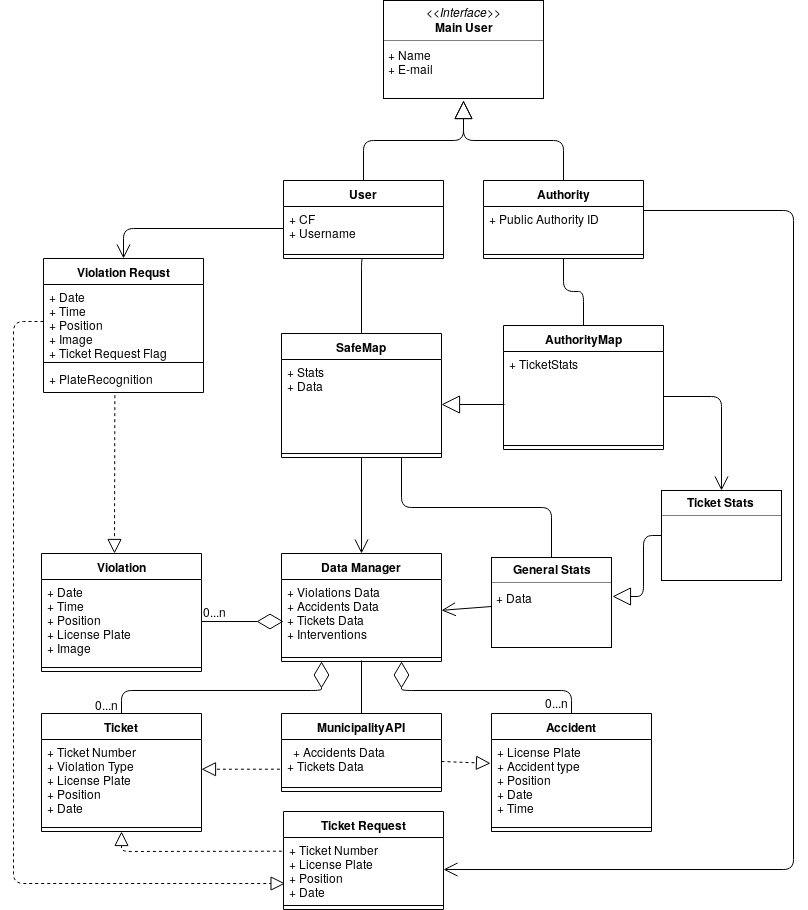
\includegraphics[scale=0.5]{Images/Diagrams/Class_Diagram.png}
				\caption{{\it SafeStreets} Class Diagram}
	\end{figure}
	
	\subsubsection{State Charts}	
	\begin{figure}[H]
				\centering
				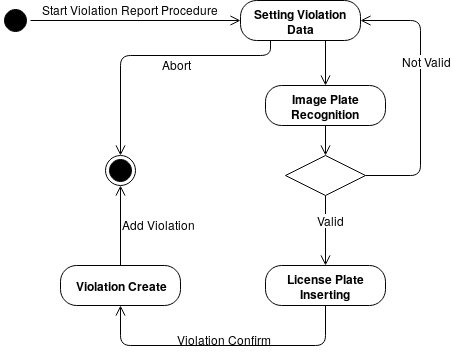
\includegraphics[scale=0.7]{Images/Diagrams/ViolationStateChart.png}
				\caption{{\it Violation Report} State Chart}
	\end{figure}
	\pagebreak
	\begin{figure}[H]
				\centering
				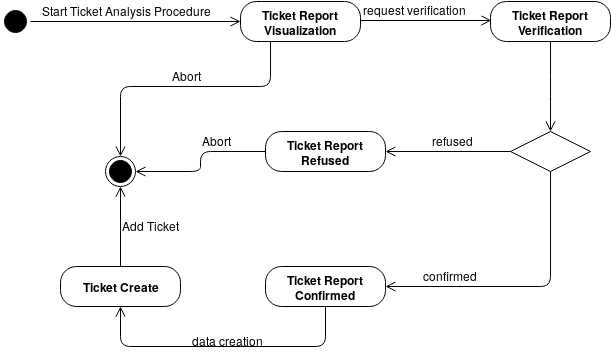
\includegraphics[scale=0.6]{Images/Diagrams/TicketStateChart.png}
				\caption{{\it Ticket Analysis} State Chart}
	\end{figure}
		

	\subsection{Product functions} 
	\begin{itemize}
	\item {\bf User Functions:} \\ \\
		{\bf Report a traffic violation} \\
		The User noticing a violation on the streets is able to, once accessed the System, fill in the information to report a violation: he takes a picture of the vehicle, with the plate decently readable, and select the type of violation from the list provided. The date, time and position are automatically taken by the system when the image is shot (the picture of the violation can only be taken using the application, not retrieved and uploaded from the photo archive) and integrated to the information given by the User. All the data is eventually sent to the System’s DBMS and the plate recognition algorithm is ran to complete the data with the plate number. If the tool fails, the User is instantly notified and asked to take a better picture. \\ \\ 
		{\bf Access statistics from notifications’ data}\\
		The User, once logged in, is able to enter the section of the application where statistics from the notifications received are available: number of violations per period (week, month, year), violations average per day of the week, the previous two per type of violation and a map showing where the violations were reported. Of course no plate number and no information about who reported the violations is shown to the User.\\ 
	\item {\bf Authority Functions:} \\ \\
		{\bf Access statistics from notifications’ data}\\
		The Municipality is able to enter the section of the system interface where statistics from the notifications received from its jurisdiction are available: number of violations per period (week, month, year), violations average per day of the week, the previous two per type of violation and a map showing where the violations were reported. The municipality can view the plate number of the offender of any violation notification but has no information on the User that reported it. \\ \\
		{\bf Obtain suggestions about unsafe areas}\\
		The system provides to the Municipality possible solutions to issues individuated through statistics, which are being mined from data on accidents and violations. This is something really valuable for the Municipality because most of the time it doesn’t have the tools itself to individuate connections and cause-effect relationship in the series of events (ex. a lot of accidents happening at a corner where a lot of second row parking violations are notified).\\ \\
		{\bf Generate tickets}\\
		The Municipality receives every notification of violations occurring under its jurisdiction and evaluates every one of them to determine whether a violation actually occurred, if the type of violation reported is correct and if there are the conditions to issue a ticket, in which case the ticket generated is no different from any ticket coming from a physically-verified violation. By exploiting the System’s information the municipality is able to issue a much larger number of tickets in its jurisdiction and to gain effectiveness in enforcing the rules. Every information about generated tickets is then shared with the System.\\ \\
		{\bf Access statistics from issued tickets}\\
		The Municipality is able to enter the section of the system interface where statistics from the tickets generated are available: number of tickets per period (week, month, year), tickets average per day of the week, the previous two per type of violation sanctioned, a map showing where the violations were reported.\\ \\
		
		
	\end{itemize}
		
	\subsection{User characteristics}
	{\it SafeStreets} has two kinds of users. There are  {\bf simple }{\it Users} of the application and {\it Authorities} (for details about the semantics about the term User refers to the section 1.3.1 of this document). The first type is usually a citizen or a tourist of the city where the {\it SafeStreets'} service is activated. The {\it User} needs to notify authorities of a violation,  and in order to do this, he/she has to install the application on his/her smartphone. The second type of user are {\it Authorities}, they are representative of the {\it Municipality}. They can access the application from their smartphone or any device supplied by the {\it Municipality}. Also their access to the service is provided by the {\it Municipality} too because they have a different level of visibility in respect to the simple {\it Users}. They need to access statistics provided by the service or have to generate tickets. \\
	The characters involved are:
	\begin{itemize}
		\item {\it Guest:} a user who has downloaded the application on his/her smartphone, but has to create an account. No functionalities can be accessed without registering to the service
		\item {\it User:} a user who has created an account, but has to log-in to access the feature. Signing-up with all the necessary data or inserting his credentials, he/she can access all the functionalities offered by the application.
		\item {\it Logged-in User:} a user who has logged-in the application providing the credentials established during the registration phase. He's able to access all the functionalities. 
		\item {\it Authorities:} a user that's a representative of the Municipality, with its own privileges and levels of visibility. Logging-in with his/her credentials, provided directly from the Municipality, there's possibility to access the functionalities.
		\item {\it Logged-in Authorities:} a user that's a representative of the Municipality, that has provided the credentials and can access all the functionalities.
	\end{itemize}
	
	\subsection{Assumptions, dependencies and constraints}
		\subsubsection{Constraints}
		\begin{itemize}
		\item {\it Users} are located on the streets under the {\it Municipality} jurisdiction when they notify the violation.
		\item {\it Users} must have a smartphone application to access the {\it System}.
		\item The {\it System} must respect the GDPR regulation.
		\item The {\it System} must ask the permission to process personal data about {\it Users}.
		\item The {\it System} must guarantee that the information is never altered during the whole process. 
		\end{itemize}
		\subsubsection{Dependencies}
		\begin{itemize}
		\item The {\it System} needs a DBMS service to retrieve and store data.
		\item The {\it System} make use of the GPS provided by the smartphone.
		\item The {\it System} uses a map visualisation service.
		\item The {\it System} make use of internet connection provided by the smartphone.
		\end{itemize}
		
		\subsubsection{Domain Assumptions}
		\begin{itemize}
		 \item {\bf [D1]} Each user, simple one or authority, has only one account.
		 \item {\bf [D2]} Data provided during the registration are correct and belong to the person who created the account
		 \item {\bf [D3]} A violation should be clearly visible and identifiable from the picture.
		 \item {\bf [D4]} A violation is processed if everything is correct, otherwise the Municipality fixes the errors.
		 \item {\bf [D5]} Data from Municipality about incidents or issued tickets are correct.
		 \item {\bf [D6]} GPS system of the device has an accuracy of 50 meters.
		 \item {\bf [D7]} Permission to access GPS and device data is granted to the System.
		 \item {\bf [D8]} Each car has a license plate.
		 \item {\bf [D9]} Municipality is entitled to issue tickets even if the violation is not physically acknowledged.
		 \item {\bf [D10]} Suggestions from the System are not discarded from the Municipality, but they are evaluated as a feasible solution.
		 \item {\bf [D11]} User takes responsibility for the reports of violation he/she submits. 
		 \end{itemize}
		
\pagebreak

% Specific Requirements - Section 3
\section{Specific Requirements}
	\subsection{External Interface Requirements}	
	\subsubsection{User Interfaces} 
	\begin{itemize} 
		\item {\bf Logo} \\
		The logo of {\it SafeStreets}, that's also the logo icon for the smartphone application, captures the value of the service provided by the application. The logo is a safe home for a car, like the idea behind the development of the application: make streets safe thanks to the notification of car violation by citizens and city's tourists.
			\begin{figure}[H]
				\centering
				
\includegraphics[height=2cm]{safestreets_logo.png}
				\caption{{\it SafeStreets} Logo}
			\end{figure}
		\item {\bf Login/Sign-up} \\
		A {\it Guest} downloads the applications and opens it for the first time. The {\it System} shows an interface that asks to choose between log-in and sign-up. If the {\it Guest} has not an account will click register to create an account in order to obtain access to all  the functionalities, while a {\it User} of the application will click login button after that he/she filled the form with his/her credentials. 
			\begin{figure} [H]
			\centering
			\begin{subfigure}{.4\textwidth}
				\centering
				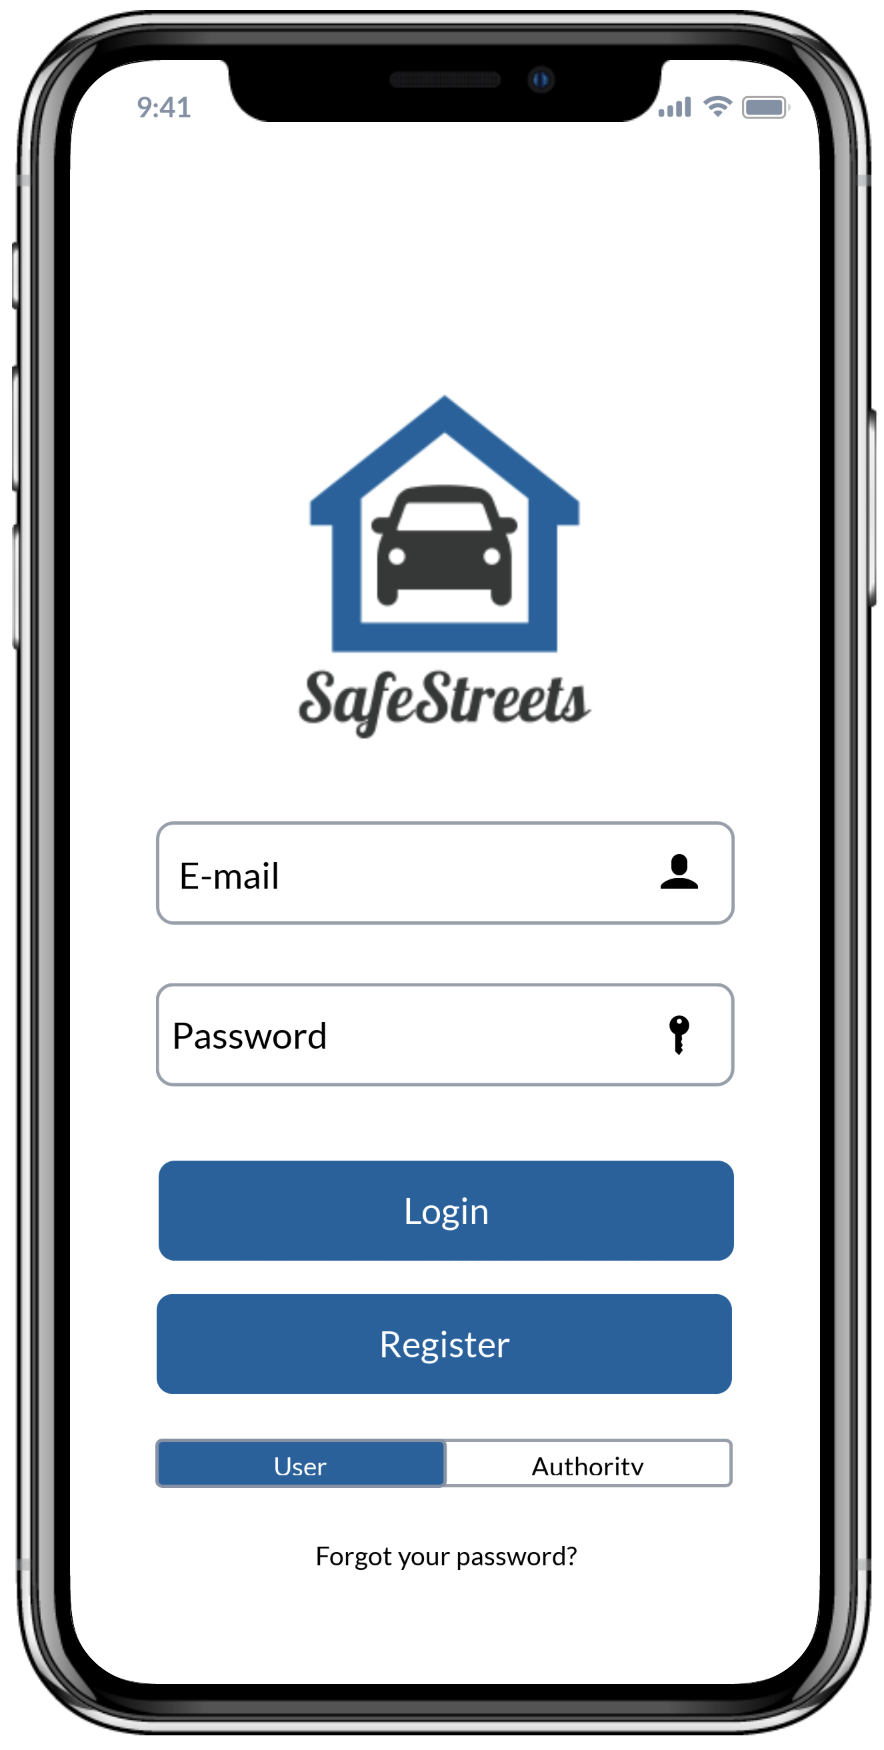
\includegraphics[height=6.2cm]{Images/Interfaces/login_user.png}
				\caption{{\it User} login}
			\end{subfigure}
			\begin{subfigure}{.4\textwidth}
				\centering
				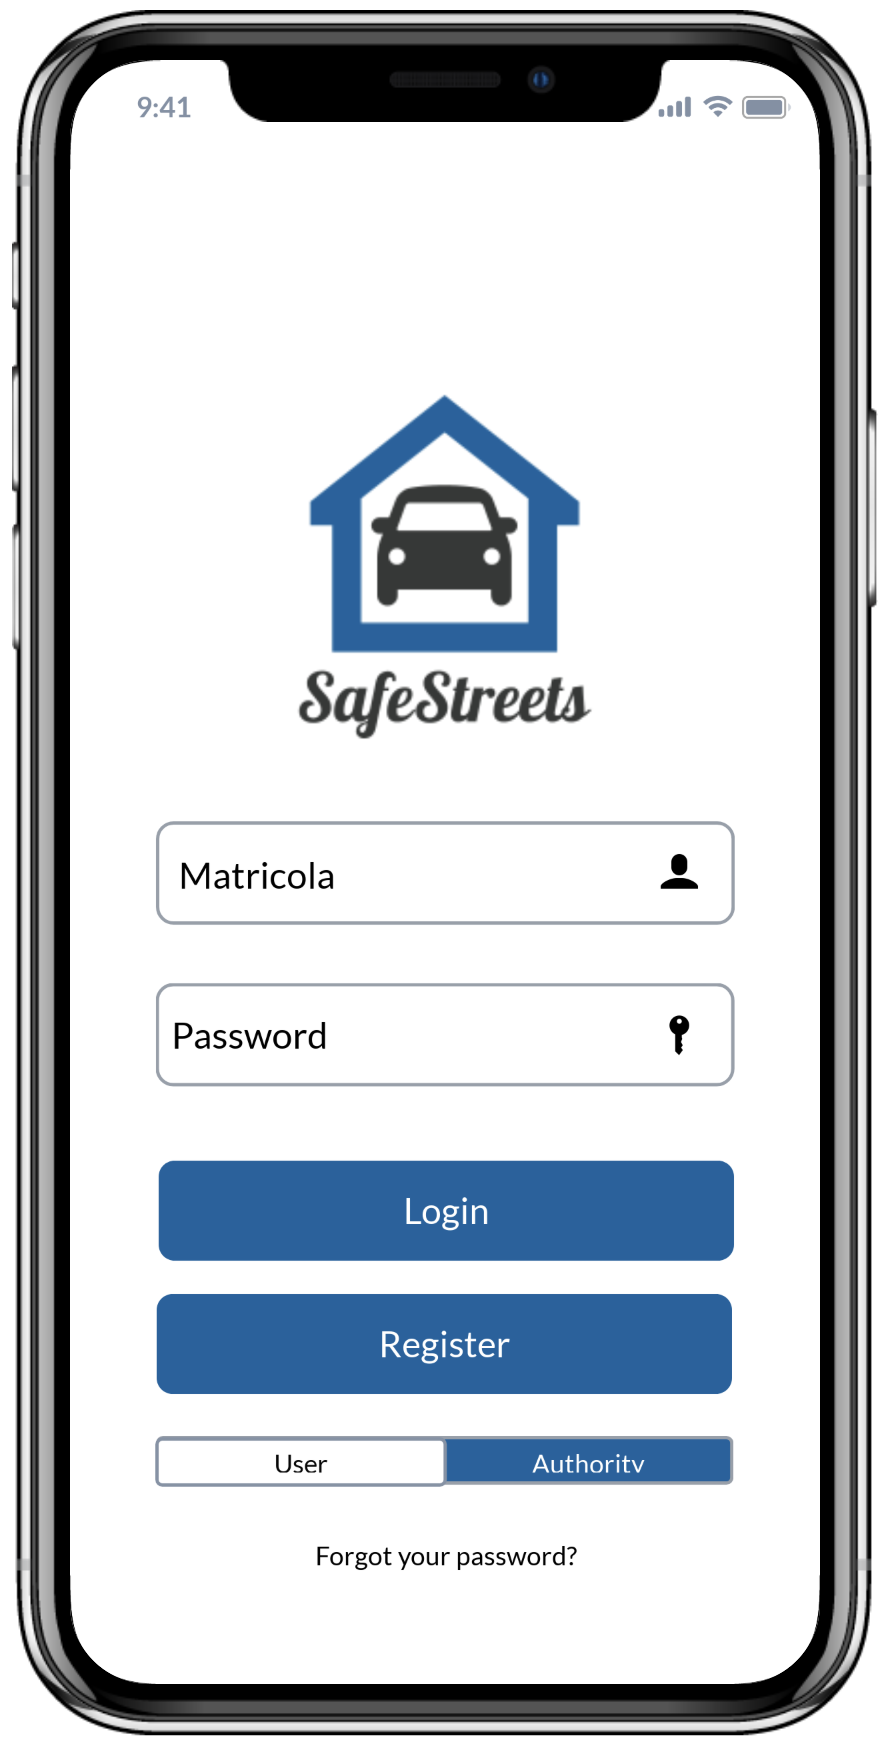
\includegraphics[height=6.2cm]{Images/Interfaces/login_auth.png}
				\caption{{\it Authority} login}
			\end{subfigure}
			\caption{Login interfaces}
			\end{figure}
			\begin{figure}[H]
			\end{figure}
		\item {\bf Account Creation} \\ 
		A {\it Guest} downloads the applications and opens it. The {\it Guest} has not an account yet, so clicks the register button. Then the {\it System} shows a form to fill with username, e-mail, password and fiscal code needed to identify the {\it User} as unique. \\
			\begin{figure} [H]
			\centering
			\begin{subfigure}{.4\textwidth}
				\centering
				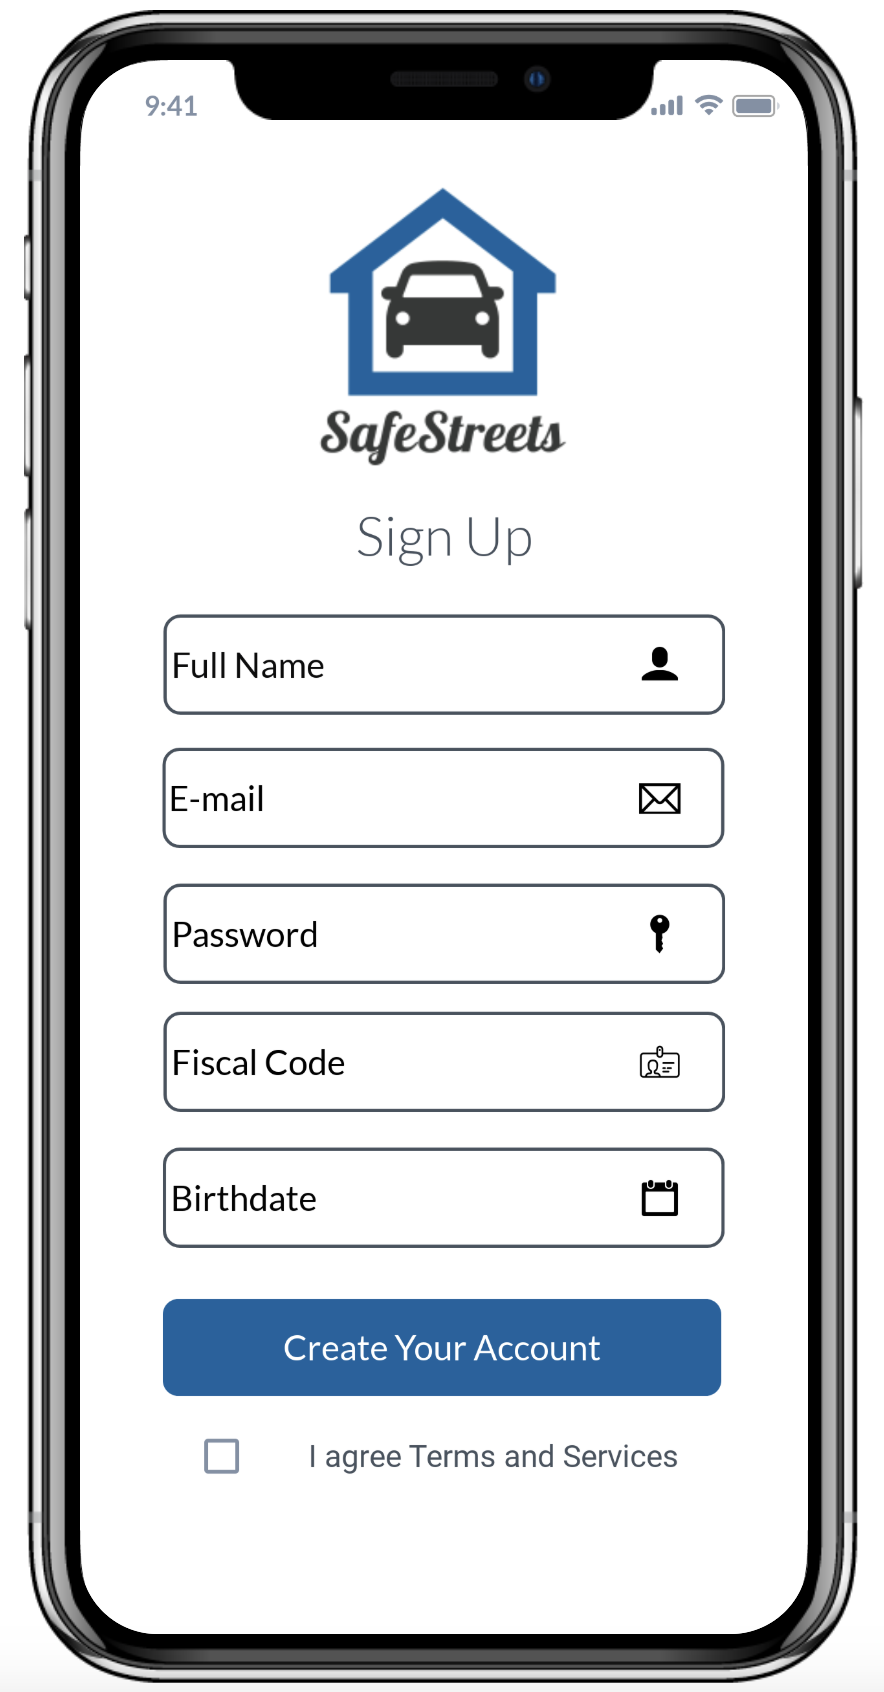
\includegraphics[height=6.2cm]{Images/Interfaces/signup.png}
				\caption{Registration form}
			\end{subfigure}
			\begin{subfigure}{.4\textwidth}
				\centering
				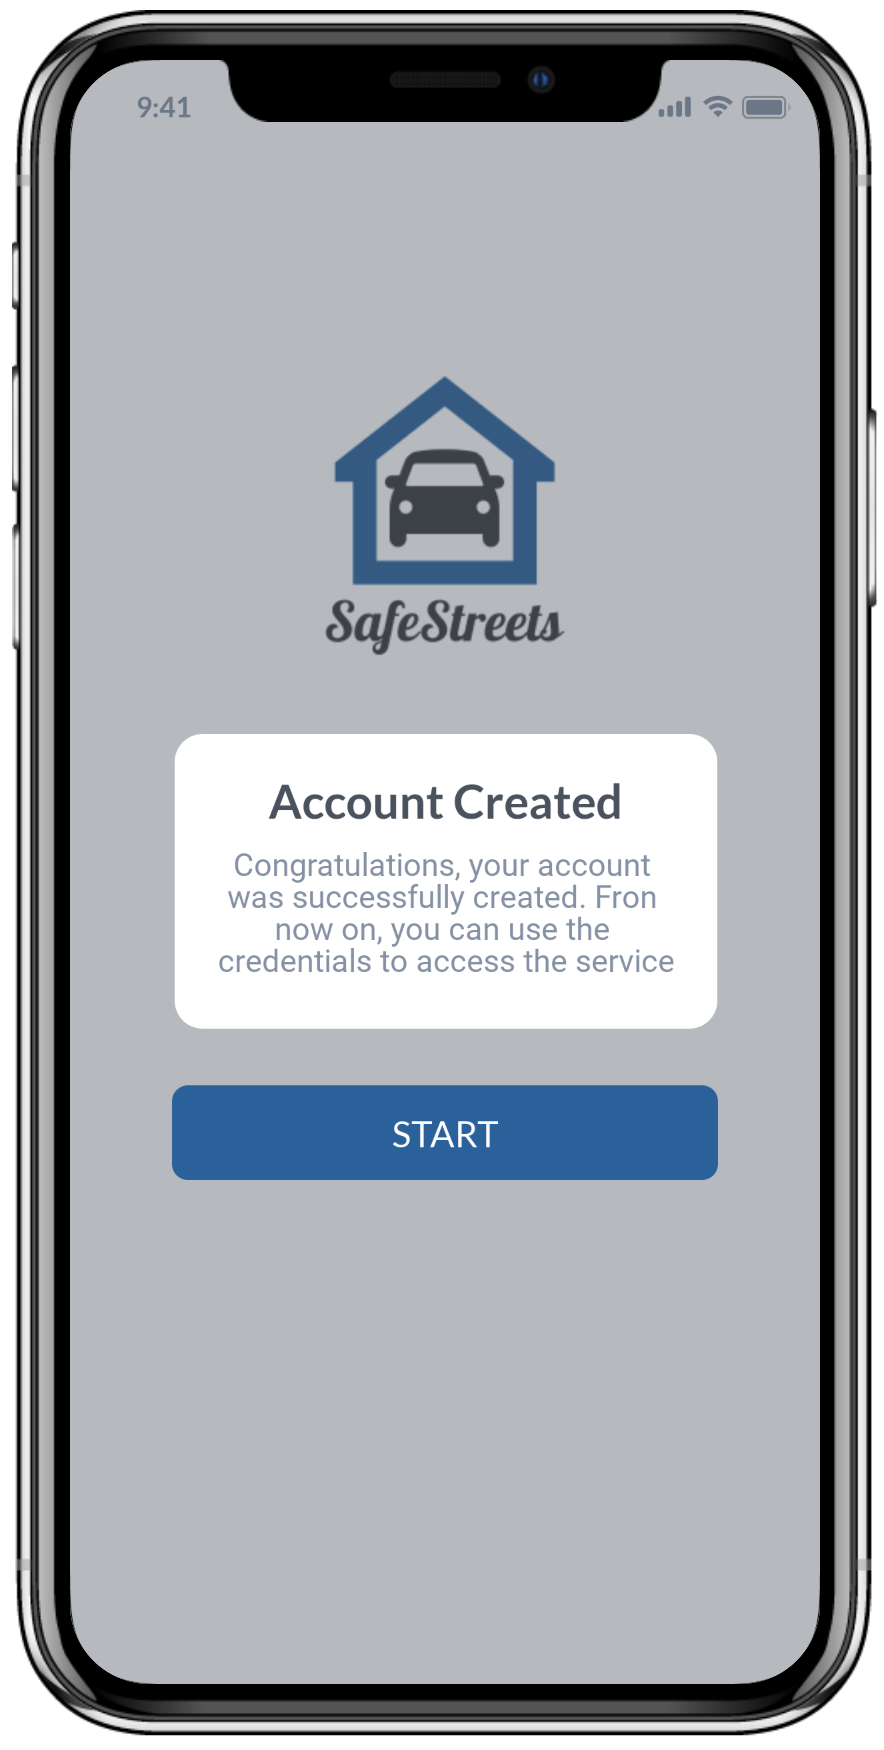
\includegraphics[height=6.2cm]{Images/Interfaces/signup_2.png}
				\caption{Registration confirmation}
			\end{subfigure}
			\caption{Account creation interfaces} 
			\end{figure}
		\item {\bf User Interface User} \\
		After the Log-in, the {\it User} enters in the application, where the {\it System} shows an interface with four tabs, each one representing a function of the application: report a violation, see the safety map, see statistics about violation and user setting. Below we will describe each section in details. 
			\begin{itemize}
			\item {\bf Report} \\
			The Report tab is the primary tab for the {\it User}. Here the {\it User} can report a violation that noticed on the streets under the {\it Municipality's} jurisdiction. He can load a picture of the violation, that will be processed by the plate recognition algorithm to be sure that the vehicle is identified and associated to the offender. From the drop down menu the {\it User} can enter the type of the violation and the date. The GPS switch should be allowed to retrieve the metadata and the position. The second interface is an alert that advise the {\it User} the report is successfully completed. 
			\begin{figure}[H]
				\centering
			\begin{subfigure}{.4\textwidth}
				\centering
				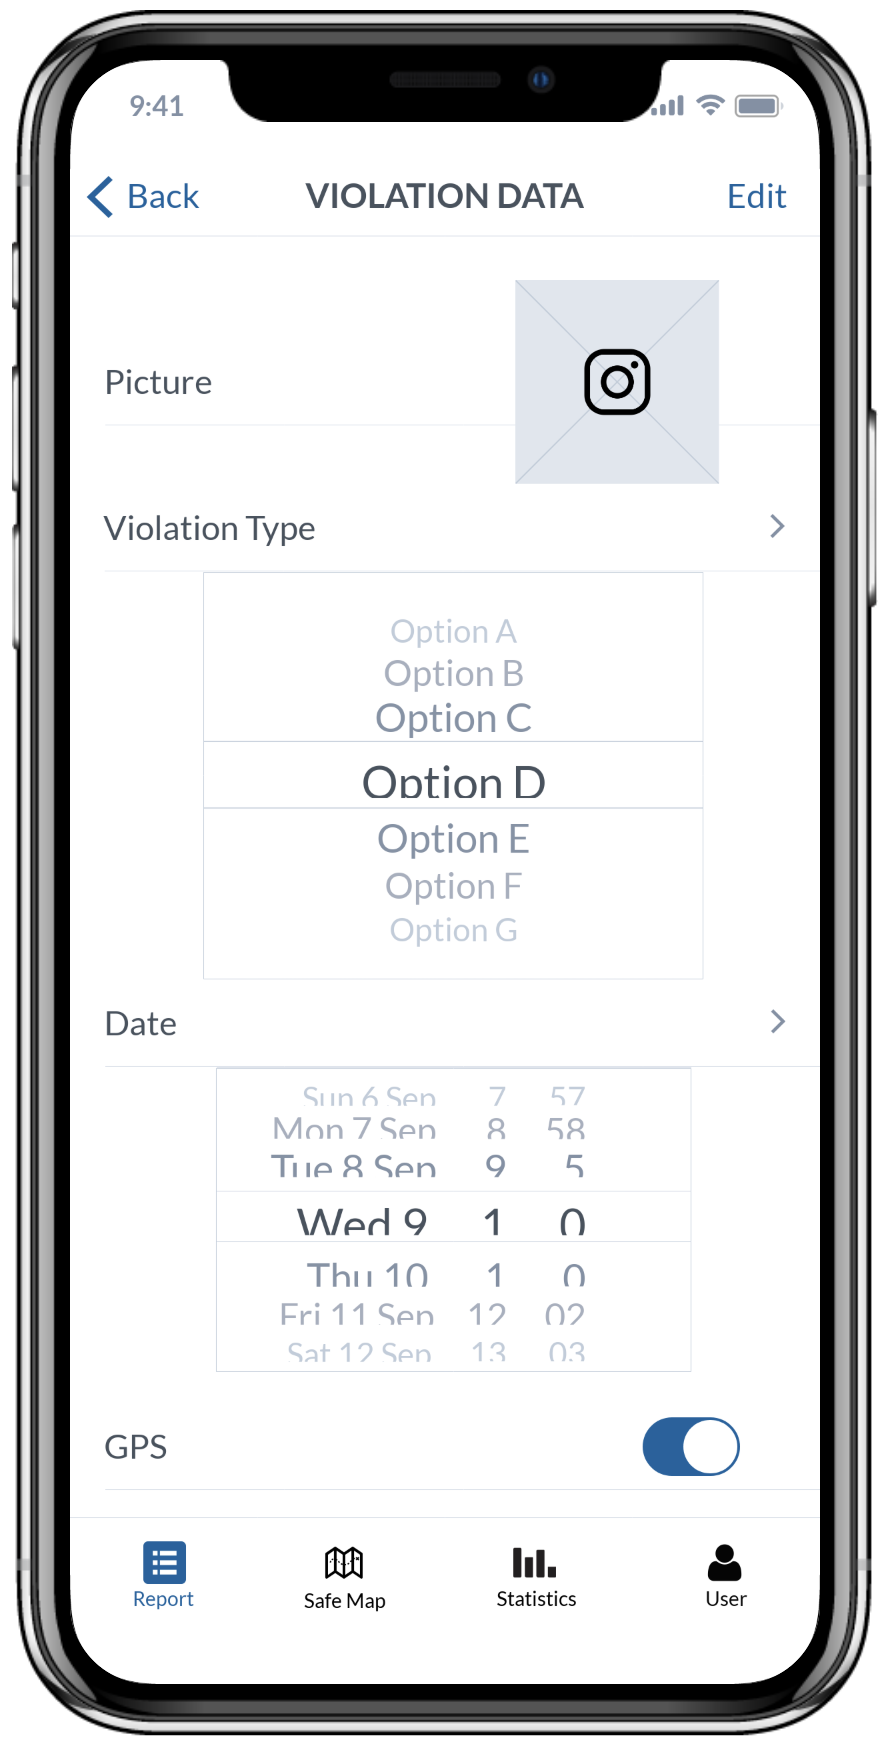
\includegraphics[height=6.2cm]{Images/Interfaces/user_report.png}
				\caption{Report violation}
			\end{subfigure}
			\begin{subfigure}{.4\textwidth}
				\centering
				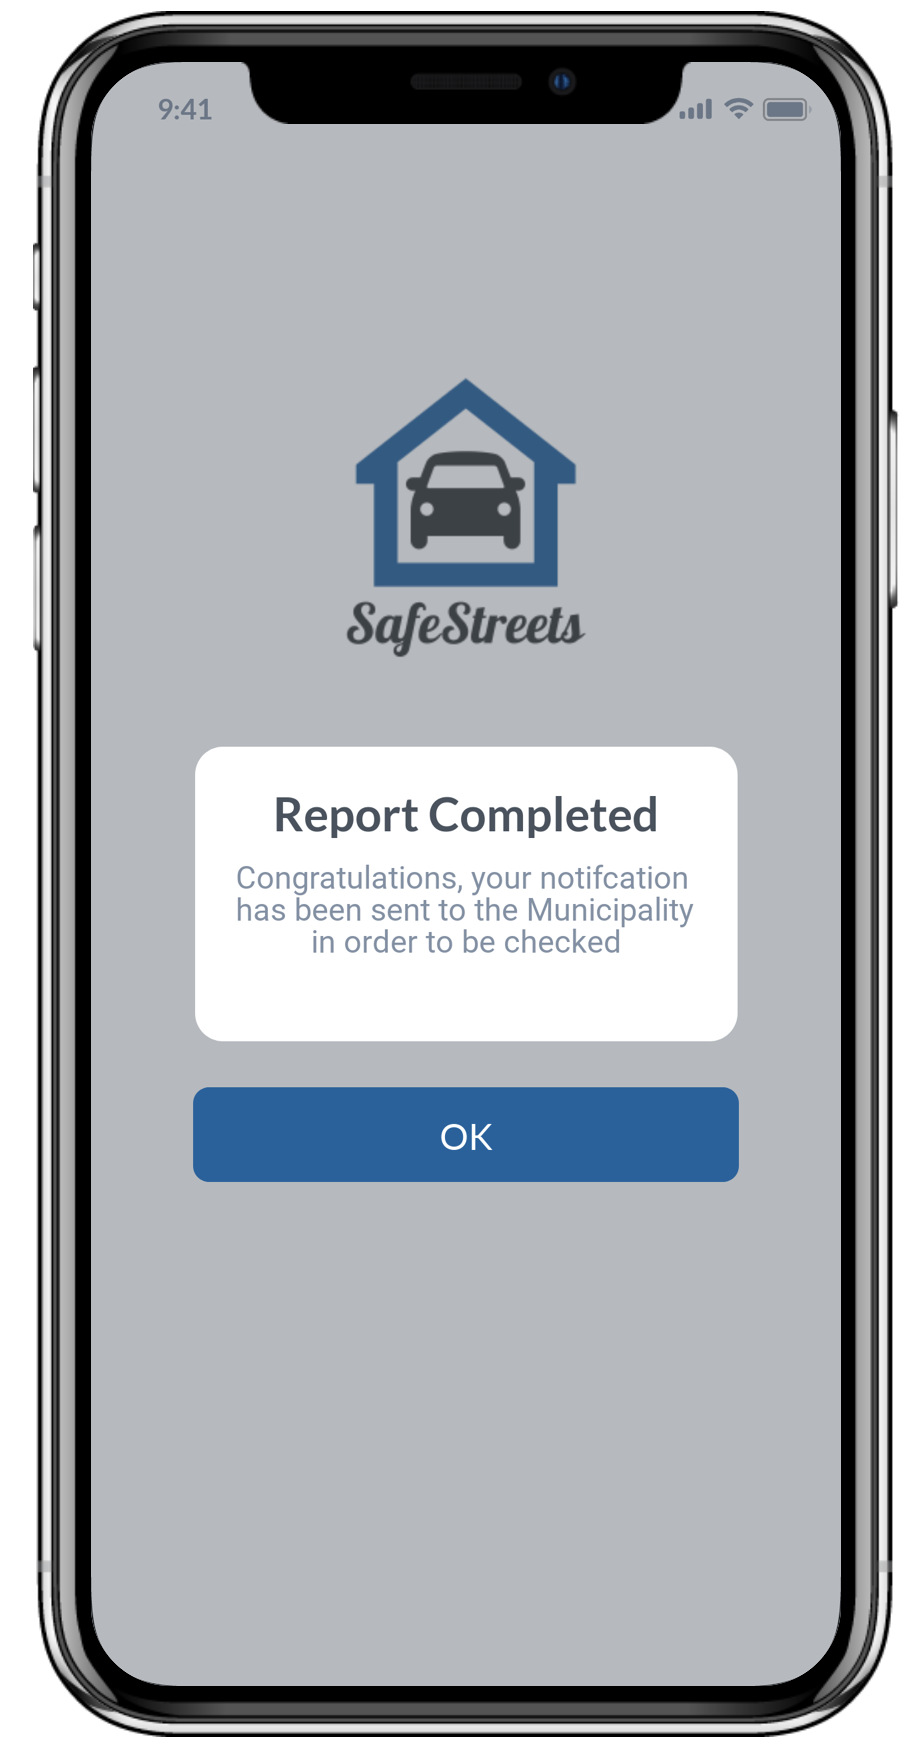
\includegraphics[height=6.2cm]{Images/Interfaces/user_report_done.png}
				\caption{Reported completed}
			\end{subfigure}
			\caption{Report Violation {\it User} Interface}
			\end{figure}

			\item {\bf Safe Map} \\
			The Safe Map tab is the second tab of the application. The {\it User} can see the map of the city where is located. The streets are highlighted with different colours (red, yellow, green). Each one indicates the violation level of the highlighted street, as stated by the legend. So, the tab give the {\it User} the possibility to access information about streets' safety. Clicking the blue points distributed on the map, the {\it User} can see the reported violation with its data.
			\begin{figure}[H]
				\centering
				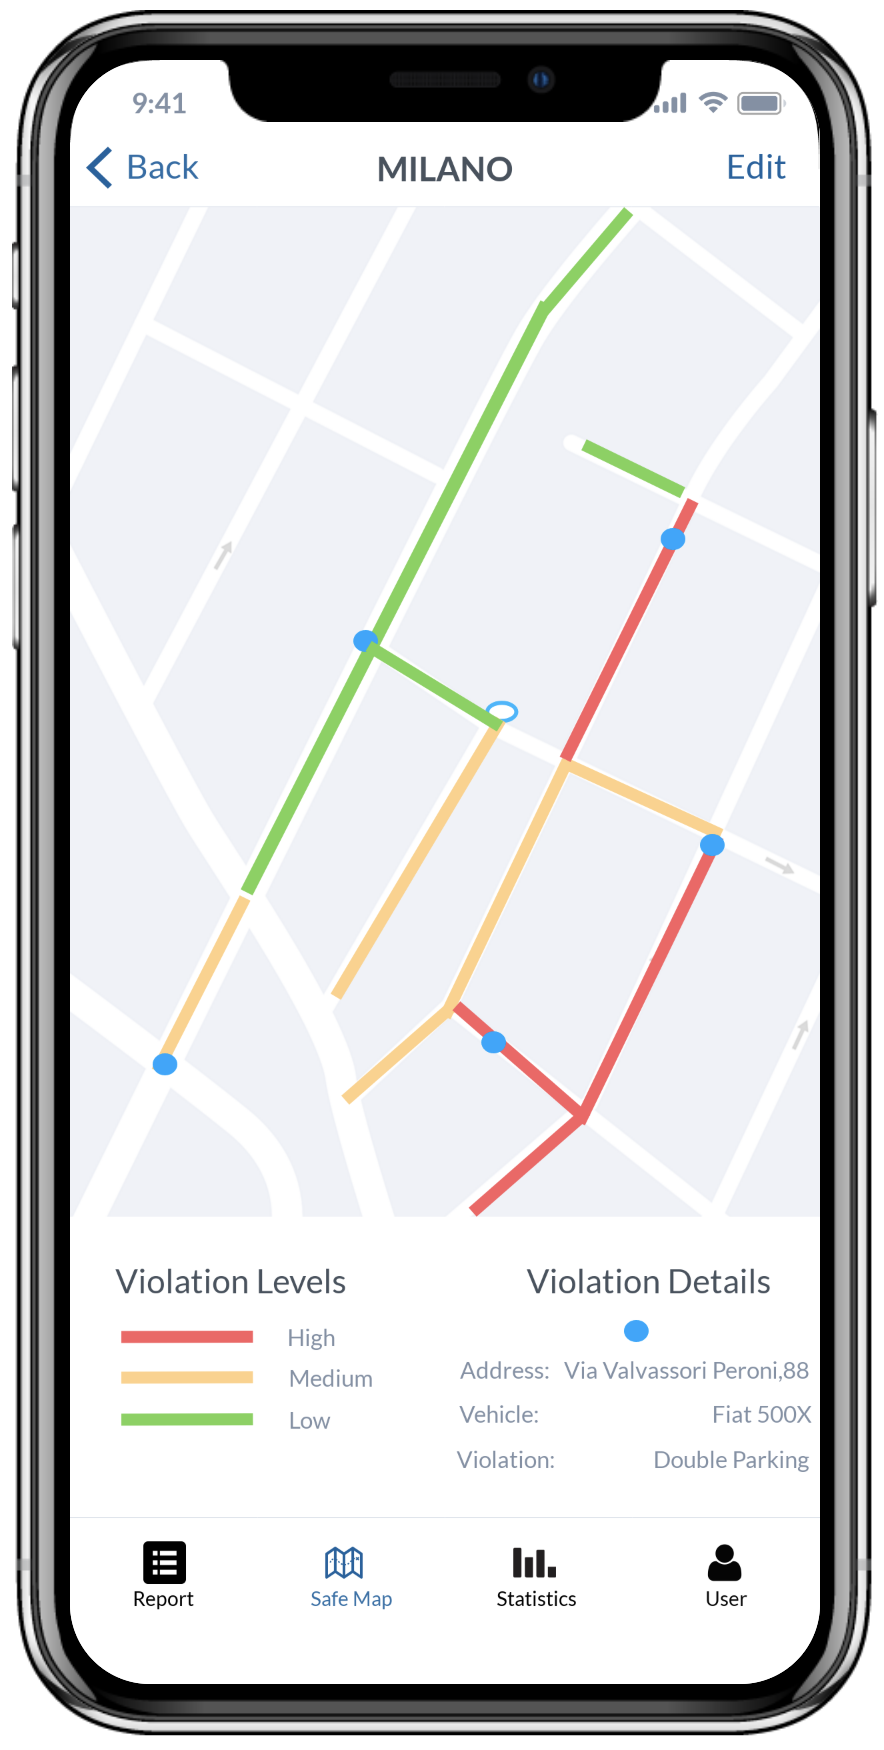
\includegraphics[height=6.2cm]{Images/Interfaces/user_map.png}
				\caption{Safe Map {\it User} interface}
			\end{figure}
			\item {\bf Statistics} \\
			The Statistics tab is the third tab of the application. The {\it User} can see the statistics obtained by the notifications' data. The interface shows some examples, such as a violation risk index of the city, the most frequent violations, the average per week day and so on and so forth. These are some of the statistics that can be generated. Others can be created and added to the same interface. 
			\begin{figure}[H]
				\centering
				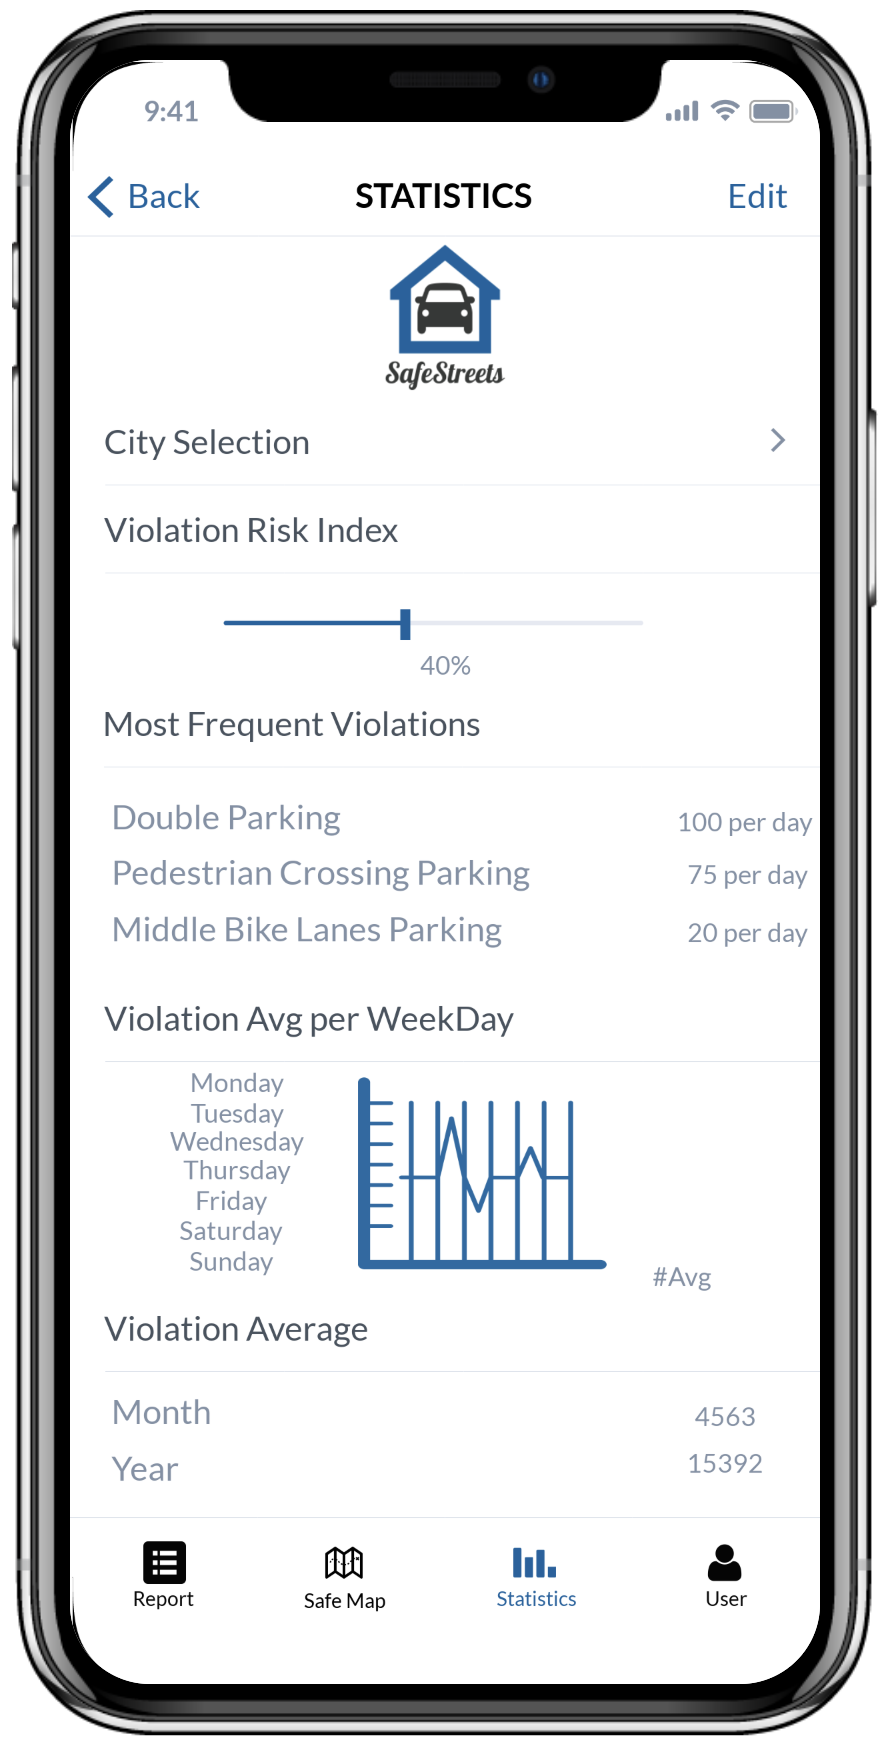
\includegraphics[height=6.5cm]{Images/Interfaces/user_stats.png}
				\caption{Statistics about violation {\it User} interface}
			\end{figure}
			\item {\bf User Settings} \\
			The User settings tab is the fourth tab of the application. It allows the {\it User} to manage personal data associated with the account. He may modify the password, name and birthdate but e-mail and fiscal code can't be changed because they are the identifiers for the {\it User}. The interface shows all the information in a list view that can be changed anytime by the {\it User}. If there's a change the {\it System} notifies the {\it User} to check the change.
			\begin{figure}[H]
				\centering
				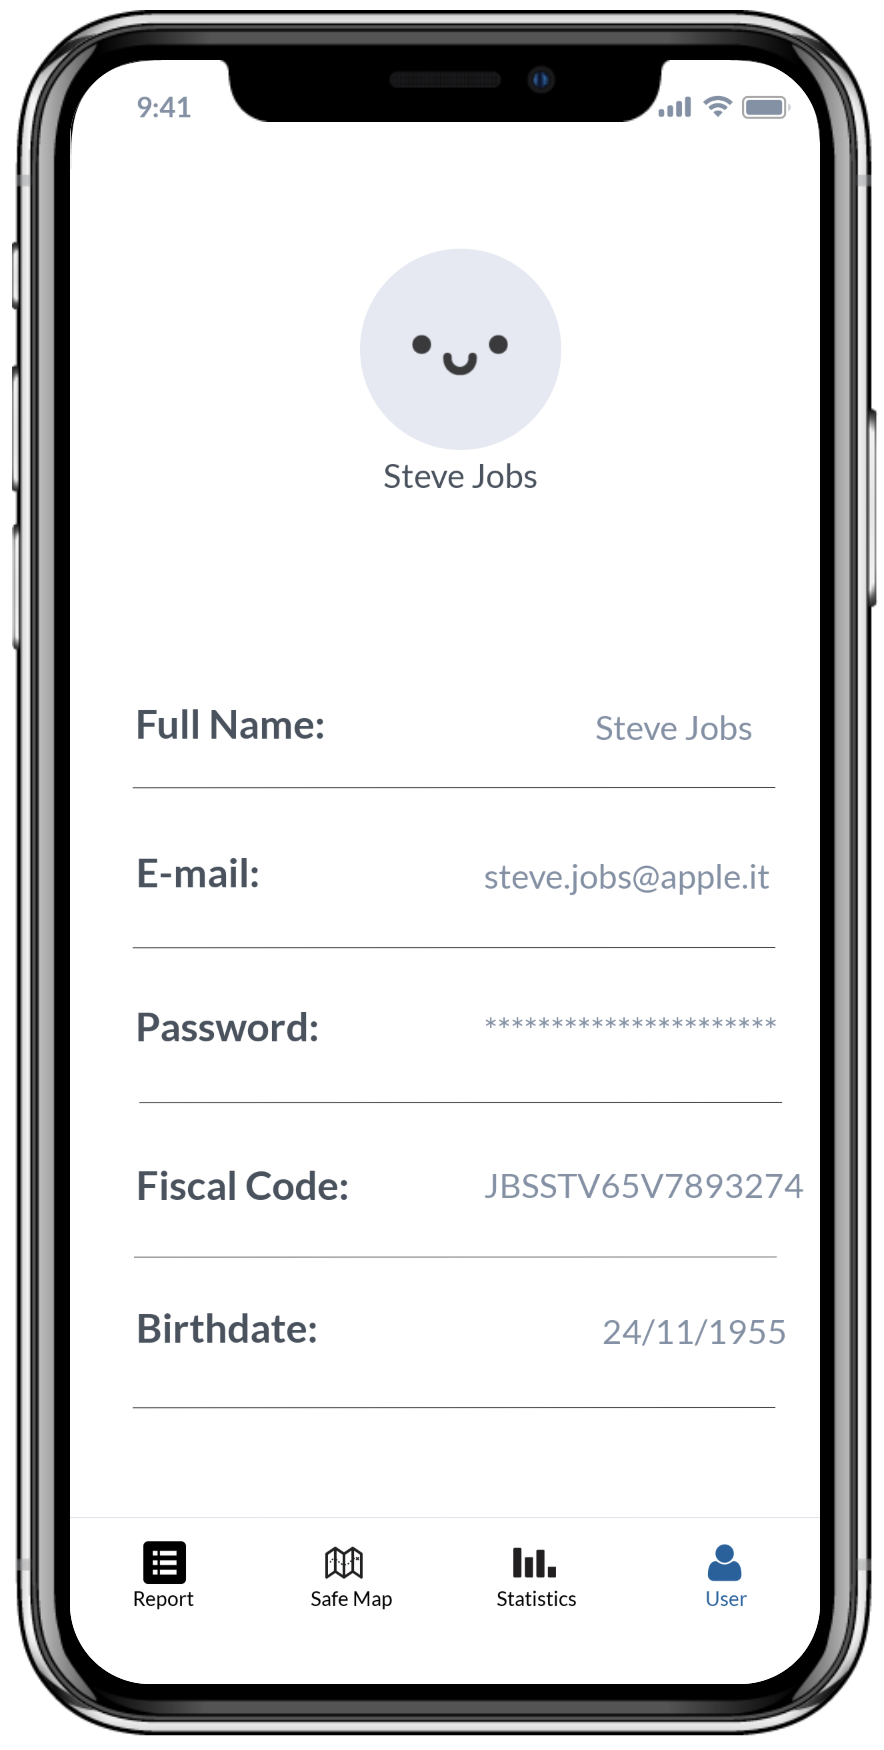
\includegraphics[height=6.2cm]{Images/Interfaces/user_settings.png}
				\caption{Settings {\it User} interface}
			\end{figure}
			\end{itemize}
		\item {\bf User Interface Authority}
			\begin{itemize}
			\item {\bf Ticket} \\
			The Ticket tab is the first tab for the {\it Authority}. The {\it Authority} can see a violation that was notified by a {\it User} on the streets. {\it Authority} can verify the picture of the violation and see all the data regarding the violation type, vehicle and owner data with a map highlighting the street where the violation happened. The {\it Authority} can decide to validate the ticket or to refuse it if it's not a traffic law violation. The second interface shows that the ticket verification has been sent. 			
			\begin{figure}[H]
				\centering
			\begin{subfigure}{.4\textwidth}
				\centering
				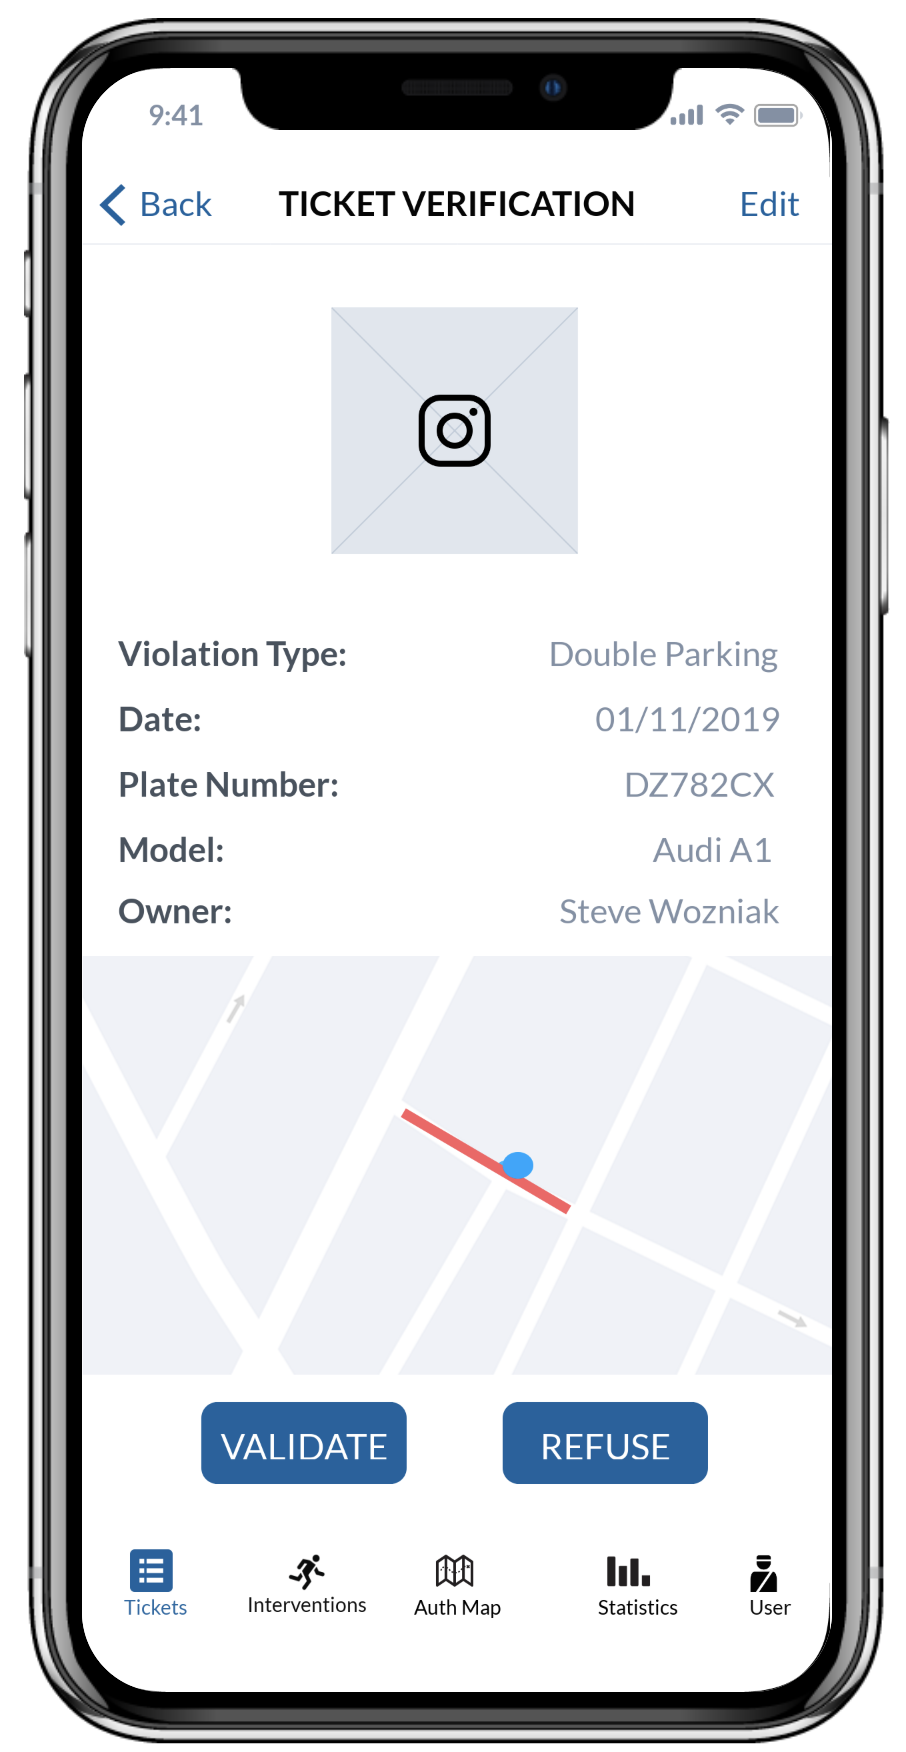
\includegraphics[height=6.2cm]{Images/Interfaces/auth_ticket.png}
				\caption{Ticket verification}
			\end{subfigure}
			\begin{subfigure}{.4\textwidth}
				\centering
				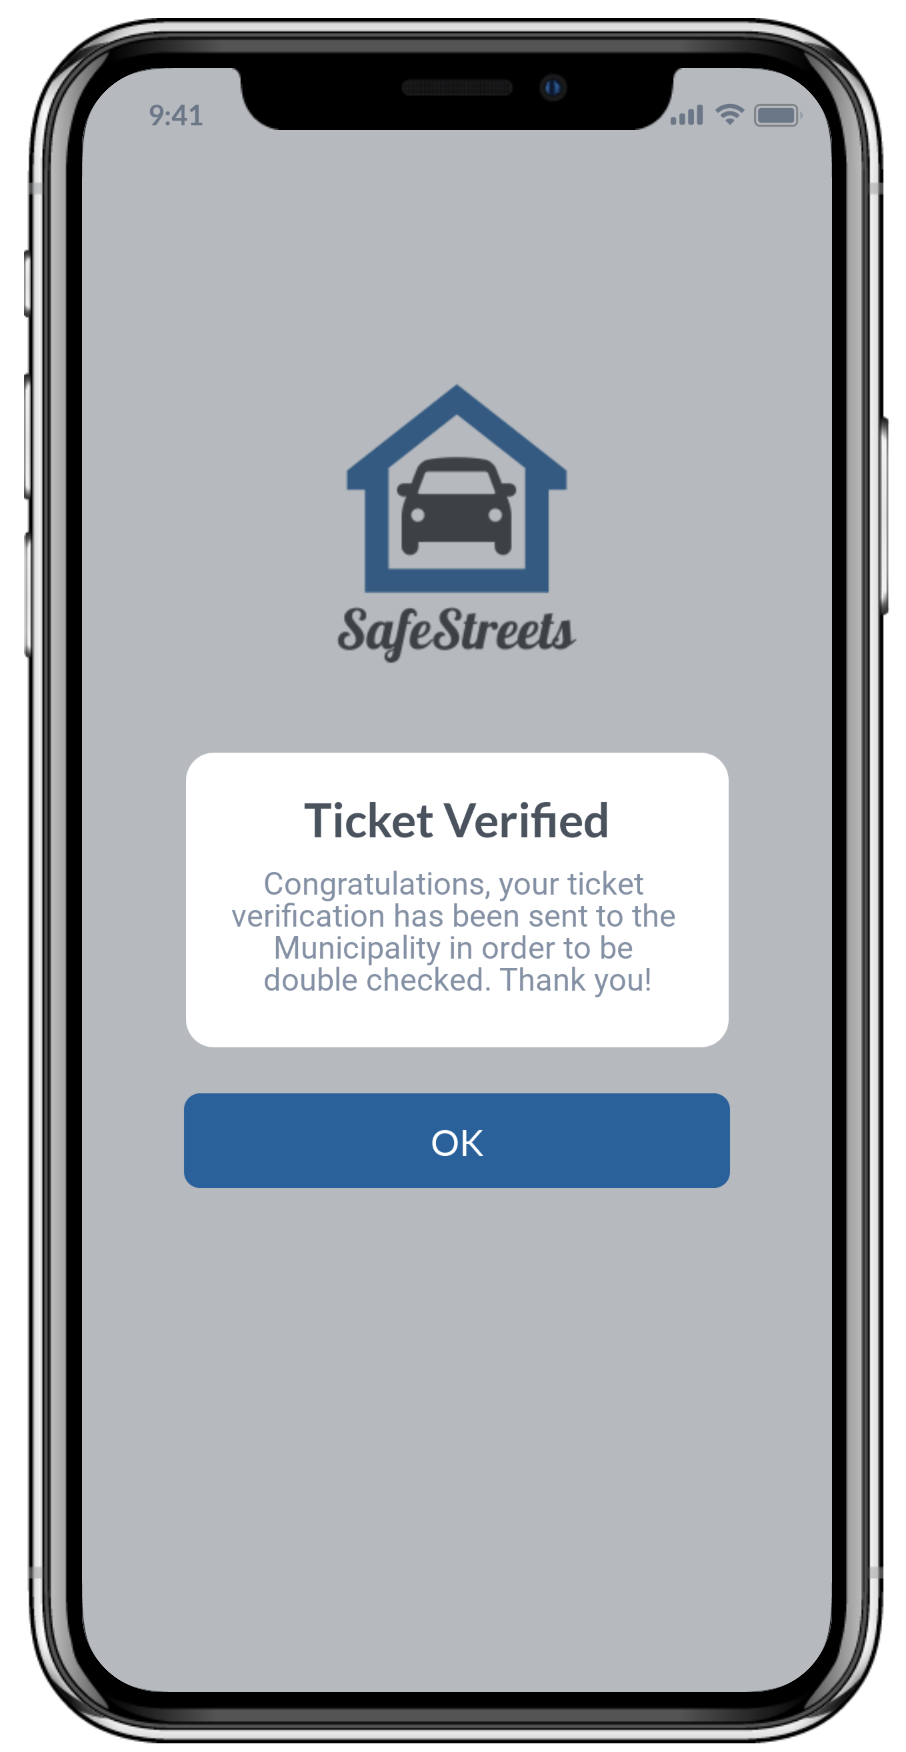
\includegraphics[height=6.2cm]{Images/Interfaces/auth_ticket_done.png}
				\caption{Ticket verification completed}
			\end{subfigure}
			\caption{Ticket Verification {\it Authority} Interface}
			\end{figure}
			\item {\bf Interventions} \\
			The Interventions is the second tab of the application. The {\it Authority} can access all the interventions suggested by {\it SafeStreets} to improve the streets' security. The {\it Authority} can select the city, see the interventions as a list with the street and a brief motivation of the suggestion. The switch button let the {\it Authority}  advise the {\it Municipality} if the {\it System} suggestion is feasible or not.
			\begin{figure}[H]
				\centering
				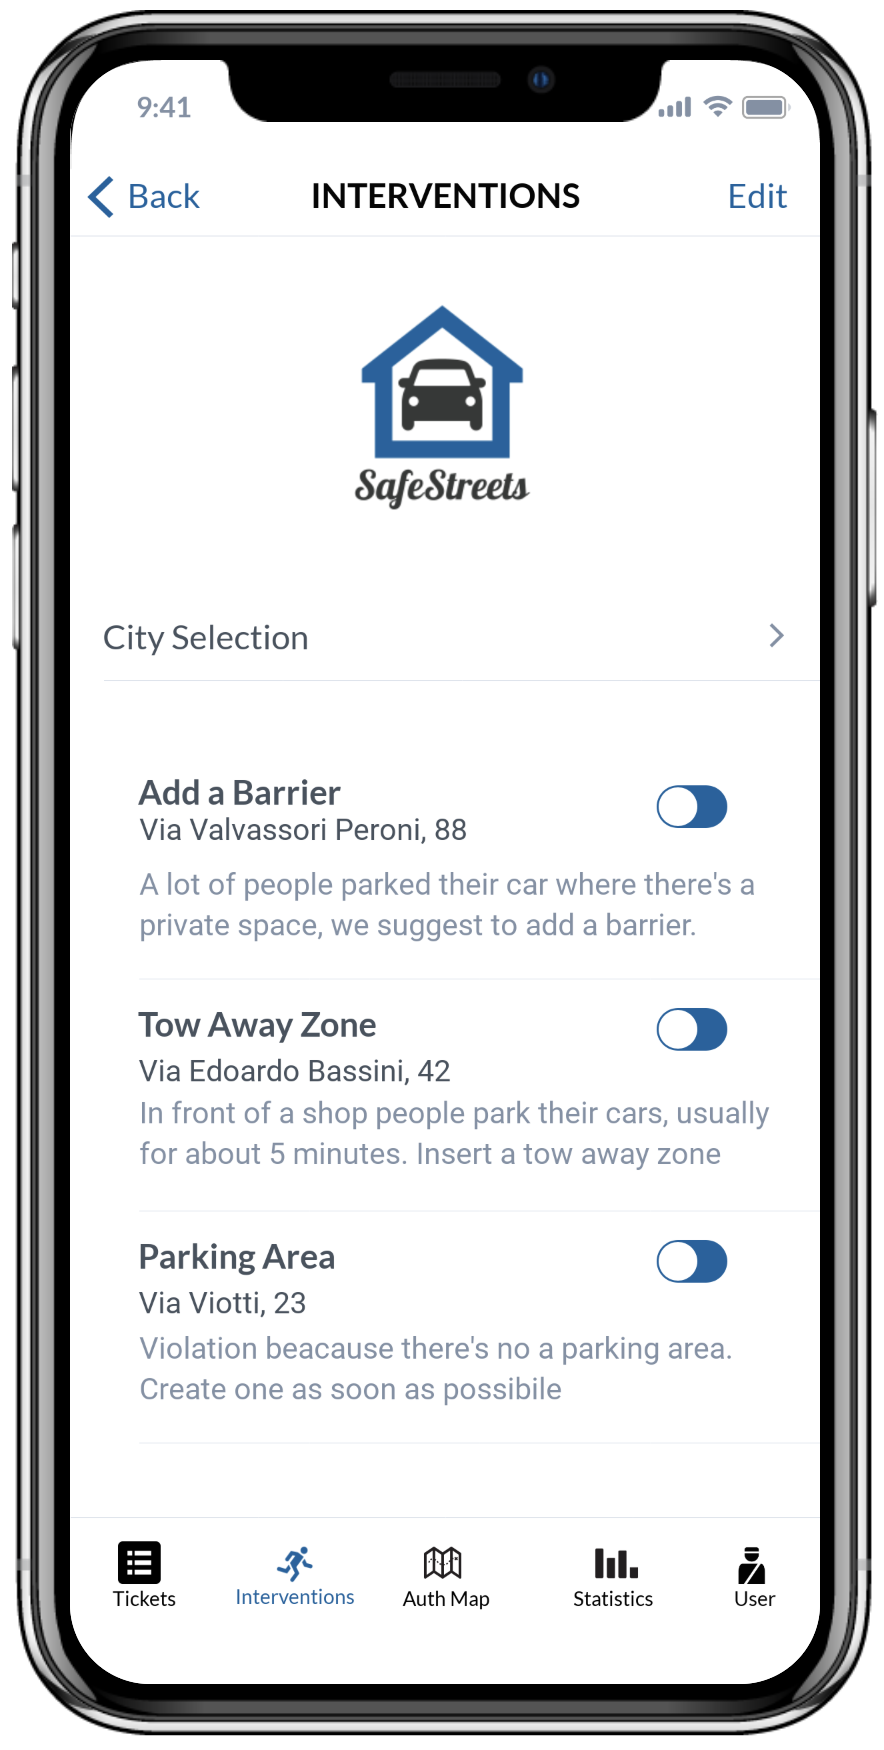
\includegraphics[height=6.2cm]{Images/Interfaces/auth_interv.png}
				\caption{Interventions {\it Authority} interface}
			\end{figure}
			\item {\bf Authority Map} \\
			The {\it Authority} Map tab is the third tab of the application. The {\it Authority} can see the map of the city where is located. The streets are highlighted with different colours (red, yellow, green). Each one indicates the violation level of the highlighted street, as stated by the legend. So, the tab give the {\it Authority} the possibility to access information about streets' safety. Clicking the blue points distributed on the map, the {\it Authority} can see the reported violation with its data and the plate number.
			\begin{figure}[H]
				\centering
				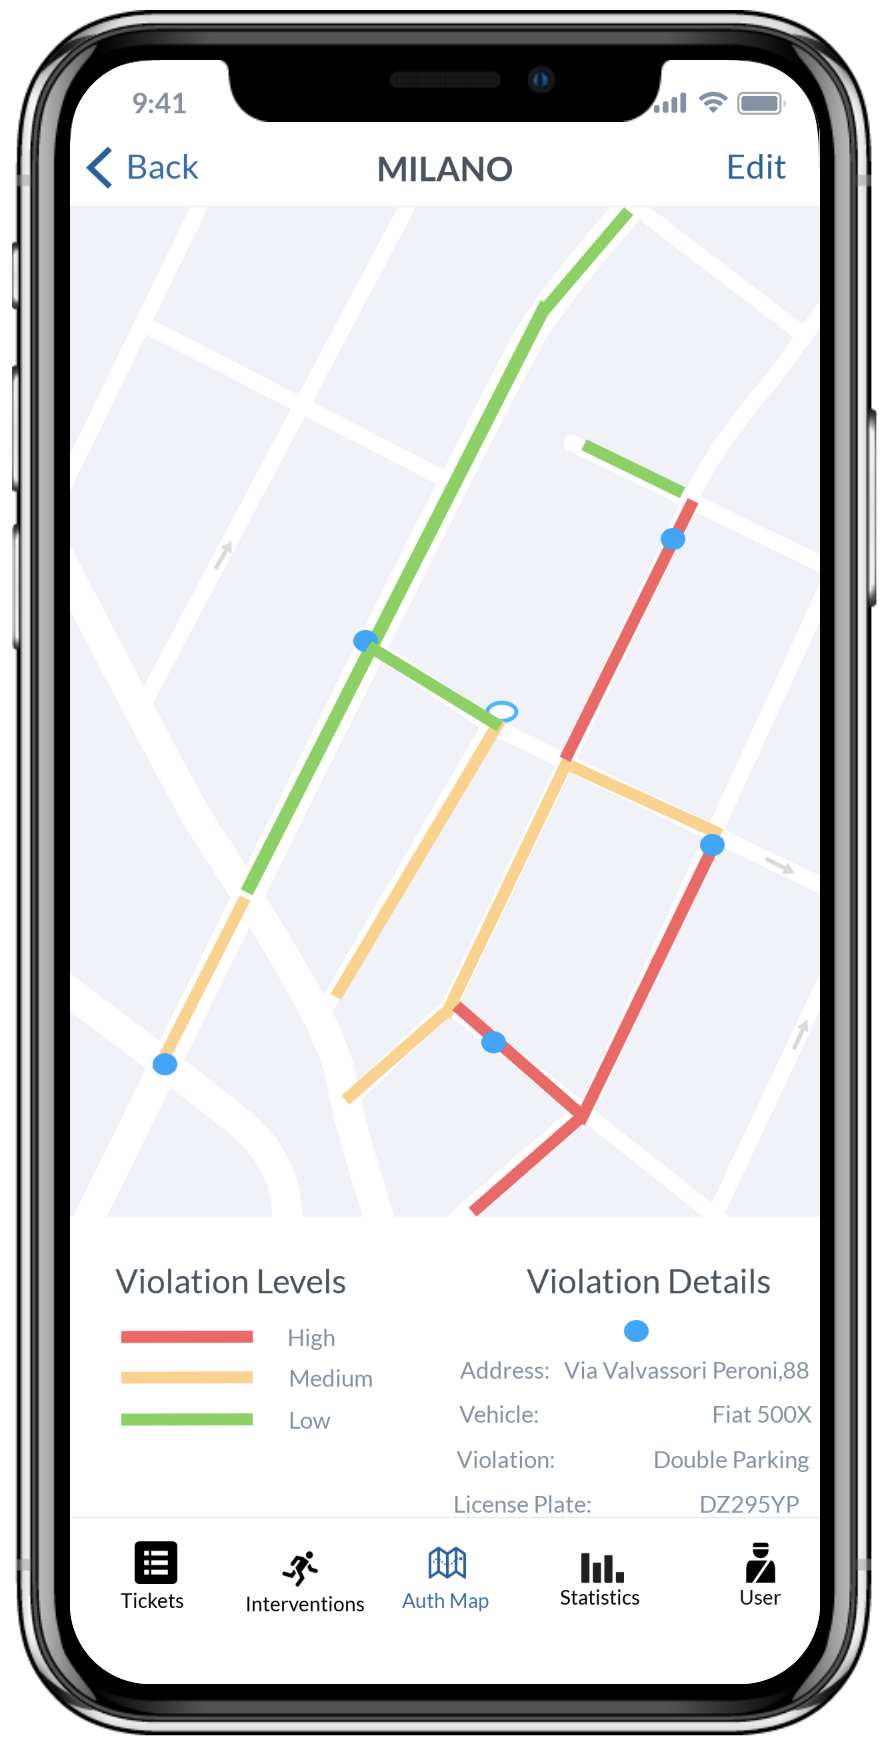
\includegraphics[height=6.2cm]{Images/Interfaces/auth_map.png}
				\caption{Map {\it Authority} interface}
			\end{figure}
			\item {\bf Statistics} \\
			The Statistics tab is the fourth tab of the application. The {\it Authority} can see the statistics obtained by the notifications' data. The interface shows some examples, such as a violation risk index of the city, the most frequent violations, the average per week day and so on and so forth. The {\it Authority} can see also the statistics derived from the tickets' data. These are just example of possible insights from data. Others can be generated and inserted in this tab. \\
				\begin{figure}[H]
				\centering
				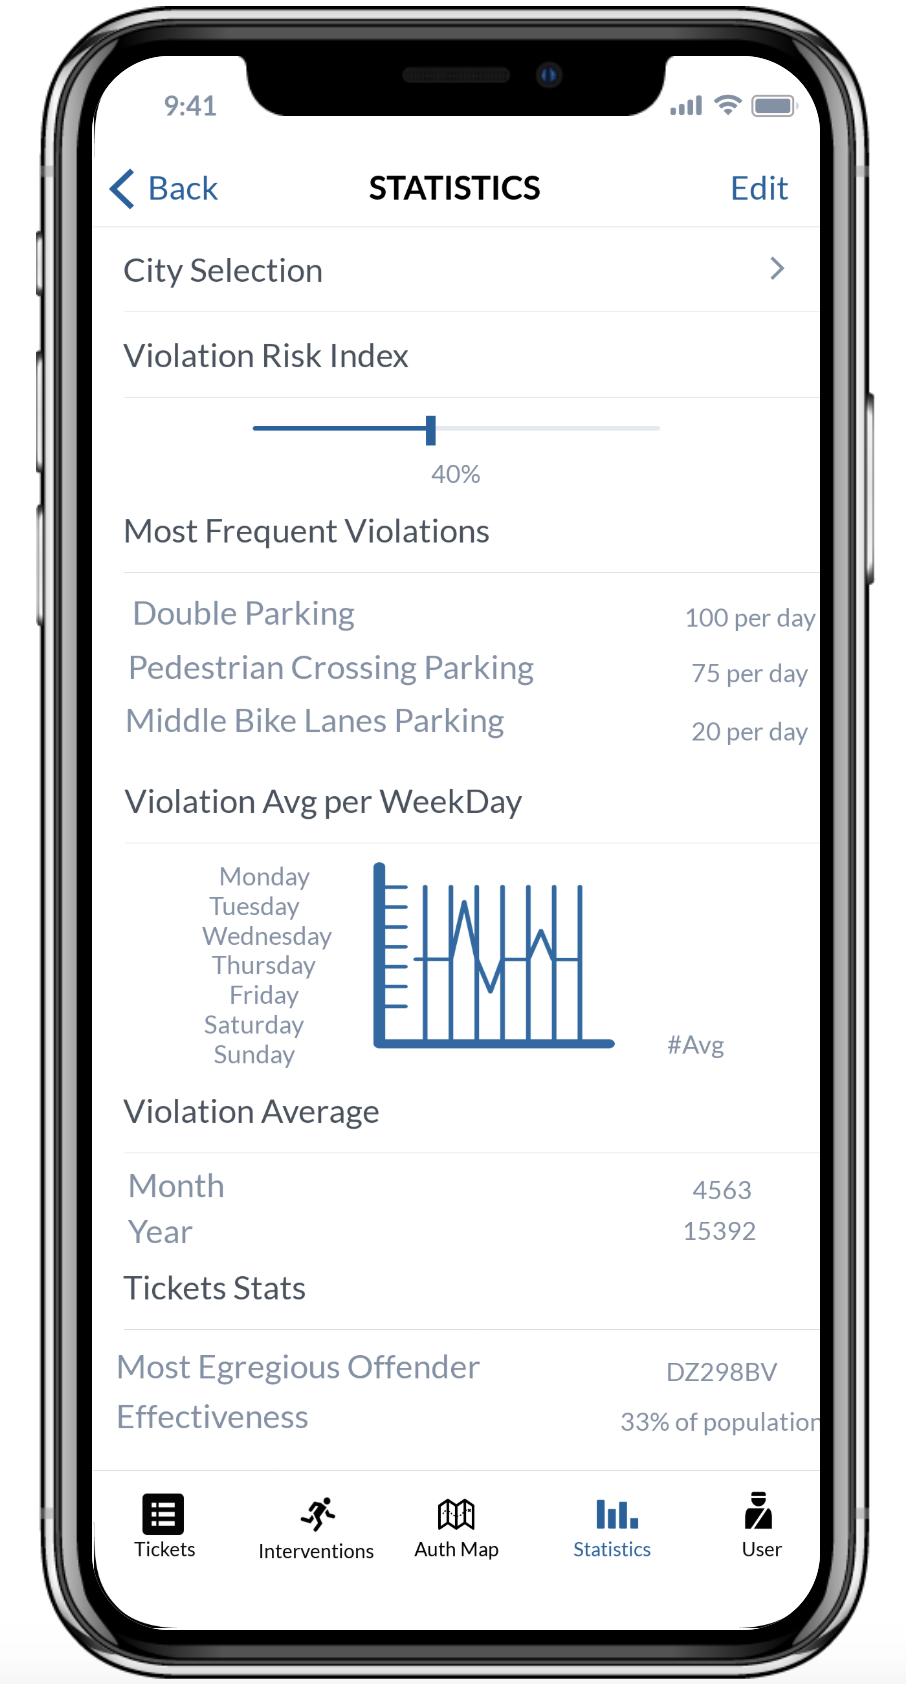
\includegraphics[height=6.5cm]{Images/Interfaces/auth_stats.png}
				\caption{Statistics {\it Authority} interface}
			\end{figure}
			\item {\bf Authority Settings} \\
			The {\it Authority} settings tab is the fifth tab of the application. It allows the {\it Authority} to manage personal data associated with the account. He may modify the password but e-mail and matricola code can't be changed because they are the identifiers given by the {\it Municipality}. The interface shows all the information in a list view.
				\begin{figure}[H]
				\centering
				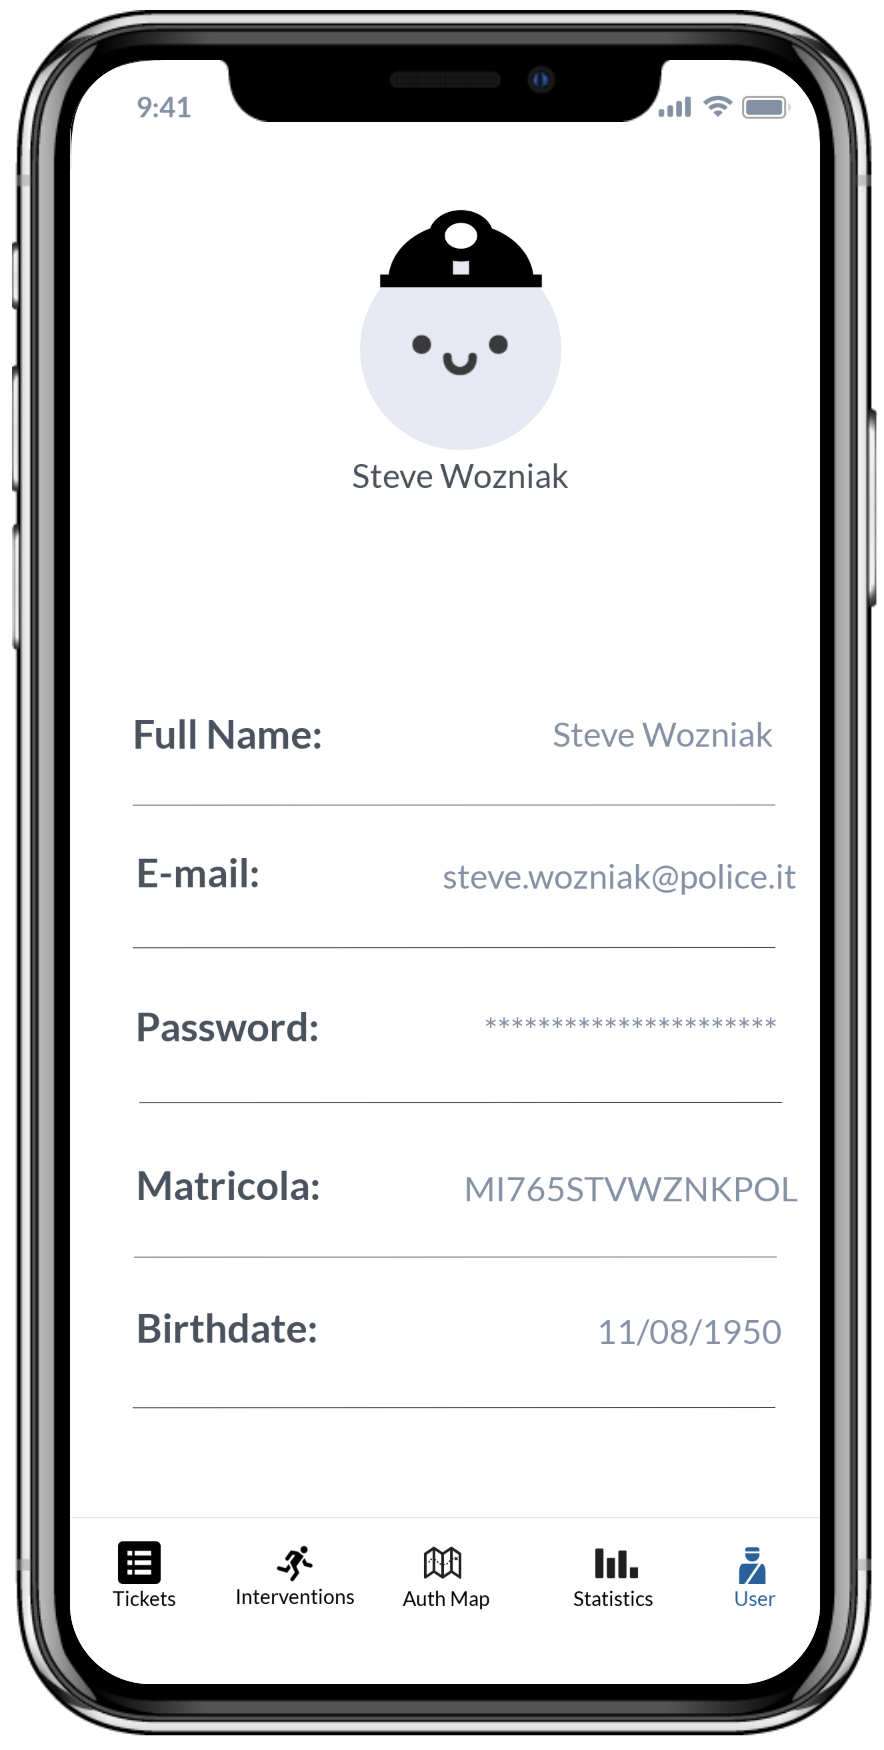
\includegraphics[height=6.5cm]{Images/Interfaces/auth_settings.png}
				\caption{Settings {\it Authority} interface}
			\end{figure}
			\end{itemize}
	\end{itemize}
	\subsubsection{Hardware Interfaces}
	The {\it SafeStreets' System} is a software application that does not offer any Hardware Interfaces, the User needs a smartphone to access the service.  
	\subsubsection{Software Interfaces}
	\begin{itemize}
		\item {\bf Operating System}
			\begin{itemize}
			\item Android
			\item iOS
			\end{itemize}
		\item {\bf Web Server}
		\item {\bf DBMS}
		\item {\bf API}: the {\it System} will use an API based communication system with external services to serve both User and Authority. Data will be exchanged in multi-platform data formats such as JSON or XML.
	\end{itemize}
	\subsubsection{Communication Interfaces}
	\begin{itemize}
		\item {\bf HTTPS Protocol:} the protocols permits a safe communication over the Internet between the application and the Web Server and/or the DBMS.
	\end{itemize}
	\subsection{Functional Requirements}
	\subsubsection{Use Case Diagrams}
	\begin{figure}[H]
				\centering
				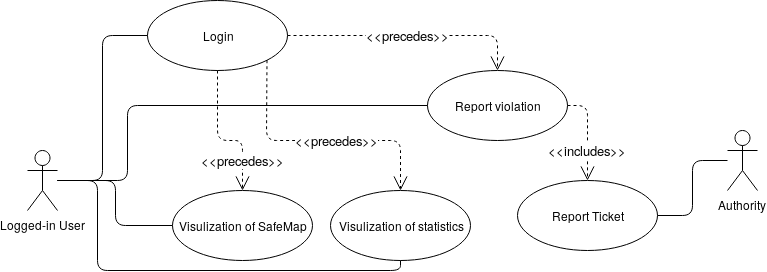
\includegraphics[scale=0.5]{Images/Diagrams/UseCaseUser.png}
				\caption{{\it User} Use Case Diagram}
	\end{figure}
	\begin{figure}[H]
				\centering
				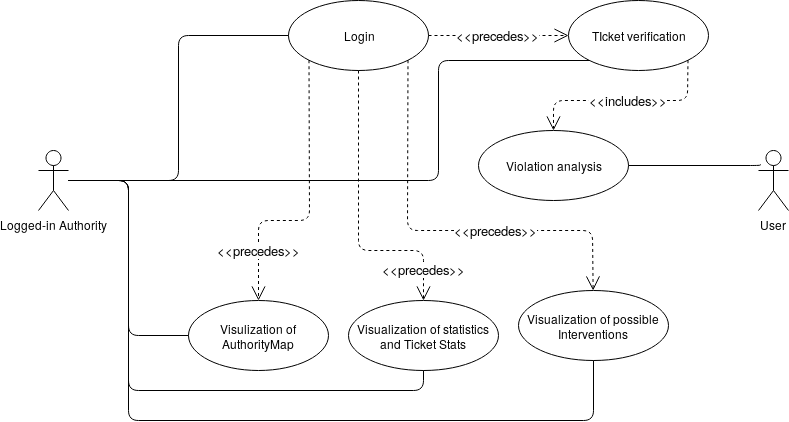
\includegraphics[scale=0.5]{Images/Diagrams/UseCaseAuthority.png}
				\caption{{\it Authority} Use Case Diagram}
	\end{figure}
	
	\subsubsection{Scenarios}
	
		{\bf Scenario 1}\\
		Marco lives next to San Siro stadium in Milan; he has been living here for 10 years now and he is used to the fact that if he needs the car in proximity and during the one or two matches that every week for most of the year are played at San Siro, he has to move it out the garage few hours in advance, park it somewhere else and most of the time even pay for the parking spot. That’s because when Inter or Milan play a game at the stadium people don’t mind using the passage at the exit of Marco’s building garages (same with every other building in the area) as it was a regular parking spot. It’s become an usual behavior because during the matches every resource of the municipality is busy providing security and traffic control right outside the stadium and along the streets that leads outside the area. It’s then very good news for Marco the announcement made by the Municipality of Milan regarding the new partnership with SafeStreets: by reporting the parking violations to the system he can make sure the offenders get sanctioned even if the authorities are busy in the exact moment of the violation, so that people will understand, ticket after ticket, to leave the car somewhere else or to go to the matches using public transportation.\\ \\
		{\bf Scenario 2}\\
		The Municipality of Pavia has to deal with an annually increasing number of car accidents causing injuries in the city center. The city council has tried to limit the traffic by setting up a limited traffic area in which most of the vehicles cannot enter in certain time slots, and that is pretty effective in reducing congestion and improving safety. However the accidents problem is just slightly affected by the measure, especially when traffic limitations are not in force. The municipality then partners with SafeStreets and start receiving violation notification from the System, which collects them from the citizens (Users). Furthermore the Municipality makes data of all past accidents available to the System and shares details of new accidents as well. In a very few months SafeStreets is able to identify a pattern, which is that half of all accidents occurring are located in just two spots, both of them intersections, not controlled by traffic lights, between two narrow streets; these are also locations of a lot of wild parking notifications, especially sidewalks parking and pedestrian crossing parking. Moreover, most of this accidents are collision between two cars and between one car and a bike in the middle of the intersections. SafeStreets informs the Municipality of the observation and suggest a low-effort and cheap solution: placing, in proximity of the intersections, dividing posts on the edge of the sidewalk, one every one or two meters, to make it impossible to leave the car without blocking the narrow street viability. That will certainly make it a lot easier to see vehicles coming from the other way.\\ \\
		{\bf Scenario 3}
		
	\subsubsection{Use Cases}
%%%%%%%%%%%%%%%%%%%%%%%%%%%%%%%%%%%%
	\begin{longtable}{| p{3 cm} | p{10.5 cm} |} 
			\hline
			{\bf ID} & UC1 \\
			\hline
			{\bf Description} & A {\it Guest} creates a {\it User} account for the application.
			\\
			\hline
			{\bf Actors} & {\it Guest}\\
			\hline
			{\bf Preconditions} & 	
			\begin{itemize}
					\item The {\it Guest} downloaded the application on the smartphone.
					\item The {\it Guest} opens the app and does not have an account yet.
				\end{itemize}	
			\\
			\hline
			{\bf Flow of events} &	
			\begin{enumerate}
				\item The {\it Guest} opens the application.
				\item The {\it System} shows the interface to login or register.
				\item The {\it Guest} clicks the register button.
				\item The {\it System} shows a form to fill with the user personal information: username, e-mail, password, fiscal code that will be used for future logins.
				\item The {\it Guest} fills the form with all the information.
				\item The {\it System} checks if all the informations are correct.
				\item The {\it System} shows an interface to confirm the account is created. 
				\item The {\it System} sends an e-mail to the {\it Guest} to confirm the account.
				\item The {\it Guest} receives the e-mail and confirms the account.
			\end{enumerate}
			\\
			\hline
			{\bf Postconditions} & 
			\begin{itemize}
				\item The {\it Guest} is now able to sign-in as a {\it User}.
				\item The {\it System} has stored the information of a new {\it User}.
			\end{itemize}
			\\
			\hline
			{\bf Exceptions} & 	
			\begin{itemize}
				\item The {\it Guest} enters an e-mail that's associated with an existing account.
				\item The {\it Guest} enters a fiscal code that's associated with an existing account. 
			\end{itemize}
			The {\it System} shows an error message and the the flow restarts from point 4.
			\\
			\hline
			\caption{Create a {\it User} account Use Case}
			\end{longtable}

%%%%%%%%%%%%%%%%%%%%%%%%%%%%%%%%%%%%	
	\begin{longtable}{| p{3 cm} | p{10.5 cm} |} 
			\hline
			{\bf ID} & UC2 \\
			\hline
			{\bf Description} & A {\it User} logs-in to the application.\\
			\hline
			{\bf Actors} & {\it User}\\
			\hline
			{\bf Preconditions} & 	
			\begin{itemize}
				\item The {\it User} downloaded the application on the smartphone.
				\item The {\it User} has already created an account.
			\end{itemize}
			\\
			\hline
			{\bf Flow of events} &	
			\begin{enumerate}
				\item The {\it User} opens the application.
				\item The {\it System} shows the interface to login or register.
				\item The {\it User} clicks the user tab.
				\item The {\it System} shows a form to fill with the credentials.
				\item The {\it User} fills the form with e-mail and password. 
				\item The {\it User} clicks the login button.
				\item The {\it System} checks if the credentials are correct. 
			\end{enumerate}
			\\
			\hline
			{\bf Postconditions} & 
			\begin{itemize}
				\item The {\it User} is logged-in.
				\item The {\it System} shows the {\it User} interface.
			\end{itemize}
			\\
			\hline
			{\bf Exceptions} & 	
			\begin{itemize}
				\item The {\it User} selects the {\it Authority} tab entering the wrong credentials. 
				\item The {\it User} enters the wrong credentials.
			\end{itemize}
			The {\it System} shows an error message and the flow restarts from point 2. \\
			\hline
			\caption{{\it User} logs-in Use Case}
			\end{longtable}
			
%%%%%%%%%%%%%%%%%%%%%%%%%%%%%%%%%%%%	
	\begin{longtable}{| p{3 cm} | p{10.5 cm} |} 
			\hline
			{\bf ID} & UC3 \\
			\hline
			{\bf Description} & {\it Authority} logs-in to the application. \\
			\hline
			{\bf Actors} & {\it Authority} \\
			\hline
			{\bf Preconditions} & 	
			\begin{itemize}
				\item The {\it Authority} downloaded the application on the smartphone.
				\item The {\it Authority} has already been provided of an account by the {\it Municipality}.
			\end{itemize}
			\\
			\hline
			{\bf Flow of events} &	
			\begin{enumerate}
				\item The {\it Authority} opens the application.
				\item The {\it System} shows the interface to login or register.
				\item The {\it Authority} clicks the authority tab.
				\item The {\it System} shows a form to fill with the credentials.
				\item The {\it Authority} fills the form with matricola and password. 
				\item The {\it Authority} clicks the login button.
				\item The {\it System} checks if the credentials are correct. 
			\end{enumerate}
			\\
			\hline
			{\bf Postconditions} & 
			\begin{itemize}
				\item The {\it Authority} is logged-in.
				\item The {\it System} shows the {\it Authority} interface.
			\end{itemize}
			\\
			\hline
			{\bf Exceptions} & 	
			\begin{itemize}
				\item The {\it Authority} selects the {\it User} tab entering the wrong credentials.
				\item The {\it Authority} enters the wrong credentials.
			\end{itemize}
			The {\it System} shows an error message and the flow restarts from point 2.
			\\ \\
			\hline
			\caption{{\it Authority} logs-in Use Case}
			\end{longtable}

%%%%%%%%%%%%%%%%%%%%%%%%%%%%%%%%%%%%			
	\begin{longtable}{| p{3 cm} | p{10.5 cm} |} 
			\hline
			{\bf ID} & UC4 \\
			\hline
			{\bf Description} & {\it User} reports a violation \\
			\hline
			{\bf Actors} & {\it User}\\
			\hline
			{\bf Preconditions} & \begin{itemize}
								  \item The {\it User} has logged in with his credentials.
								  \item The location of the violation (therefore the {\it User's}) is within the {\it Municipality's} jurisdiction
								  \end{itemize}	\\
			\hline
			{\bf Flow of events} &	\begin{enumerate}
								  \item The {\it User} notices a traffic laws violation 
								  \item The {\it User} decides to do something about it and accesses the {\it System}.
								  \item The {\it User}, in the “Report a violation” tab, takes a picture of the violation and submits it to the {\it System}.
								  \item The {\it System} runs the plate recognition algorithm on the picture to integrate the data with the plate number.
								  \item The {\it User} selects the type of violation from the drop down menu.
								  \item The {\it User} submits the notification to the {\it System}.
								  \end{enumerate}	\\
			\hline
			{\bf Postconditions} & \begin{itemize}
								  \item The {\it System} forwards the notification to the {\it Municipality}
								  \end{itemize}	 \\
			\hline
			{\bf Exceptions} & 	\begin{itemize}
								  \item The plate of the of the vehicle involved in the violation is not recognised by the {\it System} specific tool (The {\it User} is then notified and asked to take a more readable picture).
								  \end{itemize}	\\
			\hline
			\caption{{\it User} report violation Use Case}
			\end{longtable}

%%%%%%%%%%%%%%%%%%%%%%%%%%%%%%%%%%%%	
	\begin{longtable}{| p{3 cm} | p{10.5 cm} |} 
			\hline
			{\bf ID} & UC5 \\
			\hline
			{\bf Description} & A {\it User} access to the {\it SafeMap}.\\
			\hline
			{\bf Actors} & {\it Logged-in User}\\
			\hline
			{\bf Preconditions} & 	
			\begin{itemize}
				\item The {\it User} downloaded the application on the smartphone.
				\item The {\it User} has logged into his account in {\it SafeStreet}.
			\end{itemize}
			\\
			\hline
			{\bf Flow of events} &	
			\begin{enumerate}
				\item The {\it User} opens the application.
				\item The {\it System} shows the interface to login or register.
				\item The {\it User} clicks the user tab.
				\item The {\it System} shows a form to fill with the credentials.
				\item The {\it User} fills the form with e-mail and password. 
				\item The {\it User} clicks the login button.
				\item The {\it System} checks if the credentials are correct. 
			\end{enumerate}
			\\
			\hline
			{\bf Postconditions} & 
			\begin{itemize}
				\item The {\it User} is logged-in.
				\item The {\it System} shows the {\it User} interface.
			\end{itemize}
			\\
			\hline
			{\bf Exceptions} & 	
			\begin{itemize}
				\item The {\it User} selects the {\it Authority} tab entering the wrong credentials. 
				\item The {\it User} enters the wrong credentials.
			\end{itemize}
			The {\it System} shows an error message and the flow restarts from point 2.
			\\ \\
			\hline
			\caption{{\it User} logs-in Use Case}
			\end{longtable}
			
%%%%%%%%%%%%%%%%%%%%%%%%%%%%%%%%%%%%	
	\begin{longtable}{| p{3 cm} | p{10.5 cm} |} 
			\hline
			{\bf ID} & UC6 \\
			\hline
			{\bf Description} & A {\it User} access to the {\it statistics}.\\
			\hline
			{\bf Actors} & {\it Logged-in User}\\
			\hline
			{\bf Preconditions} & 	
			\begin{itemize}
				\item The {\it User} downloaded the application on the smartphone.
				\item The {\it User} has logged into his account in {\it SafeStreet}.
			\end{itemize}
			\\
			\hline
			{\bf Flow of events} &	
			\begin{enumerate}
				\item The {\it User} opens the application.
				\item The {\it System} shows the interface to login or register.
				\item The {\it User} clicks the user tab.
				\item The {\it System} shows a form to fill with the credentials.
				\item The {\it User} fills the form with e-mail and password. 
				\item The {\it User} clicks the login button.
				\item The {\it System} checks if the credentials are correct. 
			\end{enumerate}
			\\
			\hline
			{\bf Postconditions} & 
			\begin{itemize}
				\item The {\it User} is logged-in.
				\item The {\it System} shows the {\it User} interface.
			\end{itemize}
			\\
			\hline
			{\bf Exceptions} & 	
			\begin{itemize}
				\item The {\it User} selects the {\it Authority} tab entering the wrong credentials. 
				\item The {\it User} enters the wrong credentials.
			\end{itemize}
			The {\it System} shows an error message and the flow restarts from point 2.
			\\ \\
			\hline
			\caption{{\it User} logs-in Use Case}
			\end{longtable}
			
%%%%%%%%%%%%%%%%%%%%%%%%%%%%%%%%%%%%	
	\begin{longtable}{| p{3 cm} | p{10.5 cm} |} 
			\hline
			{\bf ID} & UC7 \\
			\hline
			{\bf Description} & An {\it Authority} access to the {\it AuthorityMap}.\\
			\hline
			{\bf Actors} & {\it Logged-in Authority}\\
			\hline
			{\bf Preconditions} & 	
			\begin{itemize}
				\item The {\it Authority} downloaded the application on the smartphone.
				\item The {\it Authority} has logged into his account in {\it SafeStreet}.
			\end{itemize}
			\\
			\hline
			{\bf Flow of events} &	
			\begin{enumerate}
				\item The {\it User} opens the application.
				\item The {\it System} shows the interface to login or register.
				\item The {\it User} clicks the user tab.
				\item The {\it System} shows a form to fill with the credentials.
				\item The {\it User} fills the form with e-mail and password. 
				\item The {\it User} clicks the login button.
				\item The {\it System} checks if the credentials are correct. 
			\end{enumerate}
			\\
			\hline
			{\bf Postconditions} & 
			\begin{itemize}
				\item The {\it User} is logged-in.
				\item The {\it System} shows the {\it User} interface.
			\end{itemize}
			\\
			\hline
			{\bf Exceptions} & 	
			\begin{itemize}
				\item The {\it User} selects the {\it Authority} tab entering the wrong credentials. 
				\item The {\it User} enters the wrong credentials.
			\end{itemize}
			The {\it System} shows an error message and the flow restarts from point 2.
			\\ \\
			\hline
			\caption{{\it User} logs-in Use Case}
			\end{longtable}
			
%%%%%%%%%%%%%%%%%%%%%%%%%%%%%%%%%%%%	
	\begin{longtable}{| p{3 cm} | p{10.5 cm} |} 
			\hline
			{\bf ID} & UC8 \\
			\hline
			{\bf Description} & A {\it User} access to {\it statistics} and {\it ticket statisticks}.\\
			\hline
			{\bf Actors} & {\it Logged-in Authority}\\
			\hline
			{\bf Preconditions} & 	
			\begin{itemize}
				\item The {\it Authority} downloaded the application on the smartphone.
				\item The {\it Authority} has logged into his account in {\it SafeStreet}.
			\end{itemize}
			\\
			\hline
			{\bf Flow of events} &	
			\begin{enumerate}
				\item The {\it User} opens the application.
				\item The {\it System} shows the interface to login or register.
				\item The {\it User} clicks the user tab.
				\item The {\it System} shows a form to fill with the credentials.
				\item The {\it User} fills the form with e-mail and password. 
				\item The {\it User} clicks the login button.
				\item The {\it System} checks if the credentials are correct. 
			\end{enumerate}
			\\
			\hline
			{\bf Postconditions} & 
			\begin{itemize}
				\item The {\it User} is logged-in.
				\item The {\it System} shows the {\it User} interface.
			\end{itemize}
			\\
			\hline
			{\bf Exceptions} & 	
			\begin{itemize}
				\item The {\it User} selects the {\it Authority} tab entering the wrong credentials. 
				\item The {\it User} enters the wrong credentials.
			\end{itemize}
			The {\it System} shows an error message and the flow restarts from point 2.
			\\ \\
			\hline
			\caption{{\it User} logs-in Use Case}
			\end{longtable}
			
%%%%%%%%%%%%%%%%%%%%%%%%%%%%%%%%%%%%				
	\begin{longtable}{| p{3 cm} | p{10.5 cm} |} 
			\hline
			{\bf ID} & UC9 \\
			\hline
			{\bf Description} & The {\it Authority} converts the violation notification into a ticket \\
			\hline
			{\bf Actors} & {\it Authority}\\
			\hline
			{\bf Preconditions} & \begin{itemize}
								  \item The {\it Authority} has logged in with his credentials.
								  
								  \end{itemize}	\\
			\hline
			{\bf Flow of events} &	\begin{enumerate}
								  \item The {\it Authority} accesses the Tickets tab on the System.
								  \item The {\it System} shows to the {\it Authority} a list of notifications reported by {\it Users}.
								  \item The {\it Authority} takes under examination a notification.
								  \item The {\it Authority} recognizes the violation in the picture.
								  \item The {\it Authority} confirms the information provided by the {\it User}.
								  \item The {\it Authority} establishes the case matches the criteria needed to generate a ticket.
								  \item The {\it Authority} generates a real ticket to the vehicle reported in the violation notification.
								  \end{enumerate}	\\
			\hline
			{\bf Postconditions} & \begin{itemize}
								  \item The {\it Municipality} transmits data about the ticket to the {\it System}.
								  \end{itemize}	 \\
			\hline
			{\bf Exceptions} & 	\begin{itemize}
								  \item The picture does not show the type of violation selected by the {\it User}, but another kind (the evaluation of the violation to generate a ticket still takes place)
								  \item The picture does not actually show a violation, or the violation is not clear enough in the picture to issue a ticket (in this case no ticket is generated)
								  \end{itemize}	\\
			\hline
			\caption{{\it Authority} ticket generation Use Case}
			\end{longtable}
			
%%%%%%%%%%%%%%%%%%%%%%%%%%%%%%%%%%%%							
	\begin{longtable}{| p{3 cm} | p{10.5cm} |} 
			\hline
			{\bf ID} & UC10 \\
			\hline
			{\bf Description} & The {\it Authority} views the suggestions on possible interventions on the viability given by the {\it System}. \\
			\hline
			{\bf Actors} & {\it Authority}\\
			\hline
			{\bf Preconditions} & \begin{itemize}
								  \item The {\it User} has logged in with his credentials.
								  \item The {\it Municipality} has been sending data on accidents to the {\it System}.
								  \end{itemize}	\\
			\hline
			{\bf Flow of events} &	\begin{enumerate}
								  \item It’s time for the Authority to do the periodic evaluation of possible improvements in viability, so it goes on the Intervention tab on the System
								  \item The System shows a list of possible interventions including the location of the issue and an explanation
								  \item The Municipality evaluates the suggestions and decides to realize one of them. The Authority then checks the specific suggestion as “done”
								  \end{enumerate}	\\
			\hline
			{\bf Postconditions} & \begin{itemize}
								  \item
								  \end{itemize}	 \\
			\hline
			{\bf Exceptions} & 	\begin{itemize}
								  \item The system was not able to elaborate any specific suggestion
								  \end{itemize}	\\
			\hline
			\caption{{\it Authority} accesses to Interventions Use Case}
			\end{longtable} 
%%%%%%%%%%%%%%%%%%%%%%%%%%%%%%%%%%%%%%			

	\pagebreak
	\subsubsection{Sequence Diagrams}
	The first sequence diagram models the interaction for the creation of a new account. The actors are a {\it Guest} and the {\it System}.
		\begin{figure}[H]
			\centering
			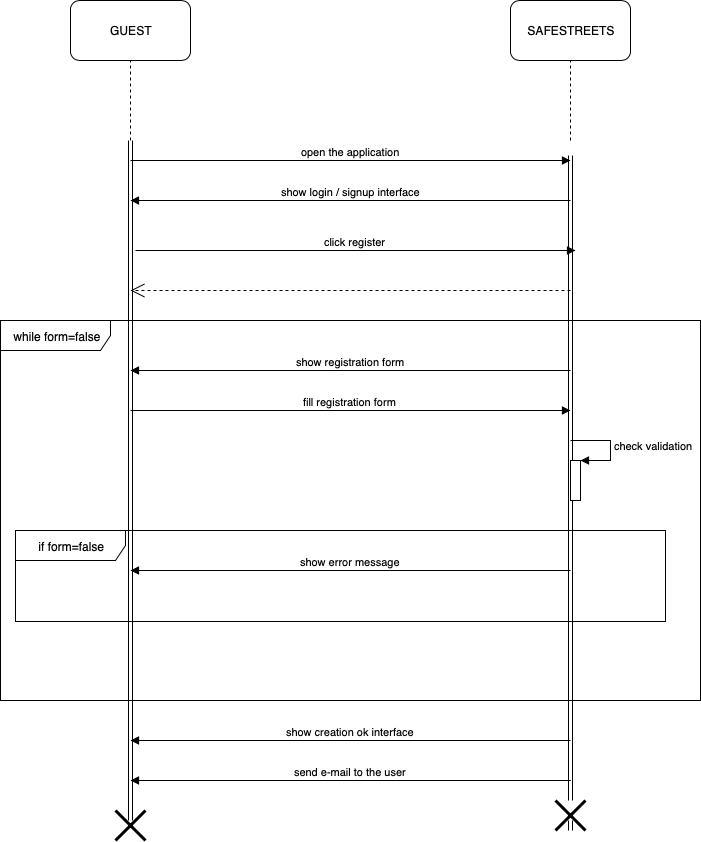
\includegraphics[scale=0.55]{images/Diagrams/sd_signup}
			\caption{Account creation sequence diagram}
		\end{figure}
	The second sequence diagram models the interaction for the log-in to the application. We created a single sequence diagram for both {\it User} and {\it Authority} because the procedure is almost the same.
		\begin{figure}[H]
			\centering
			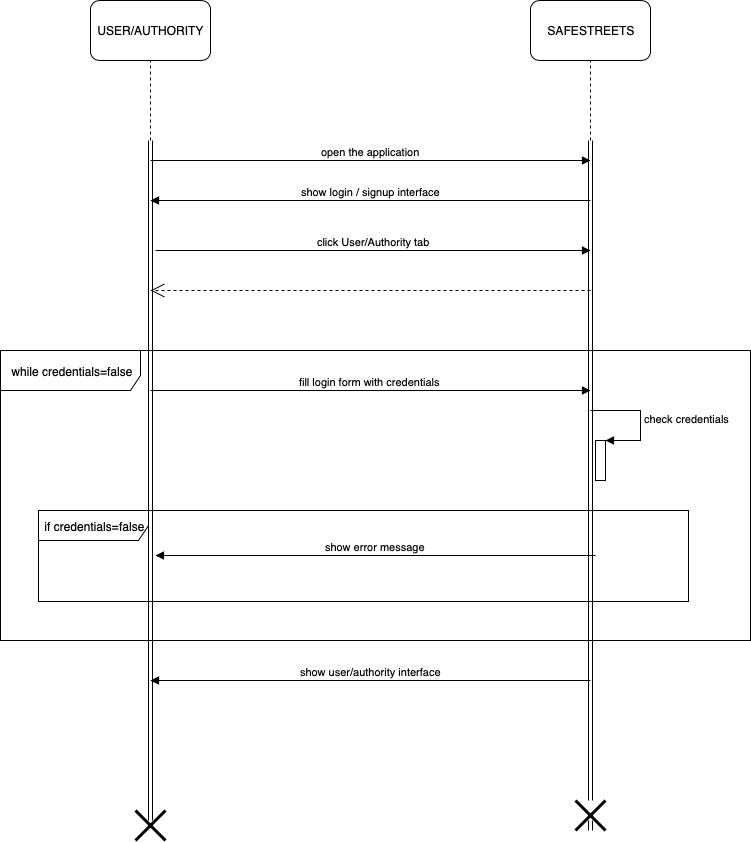
\includegraphics[scale=0.55]{images/Diagrams/sd_login}
			\caption{Application log-in sequence diagram}
		\end{figure}
	
	\subsubsection{Mapping on Requirements}
	\begin{itemize}
			 \item {\bf [G1]} The System has to be used both by {\it Users} and {\it Authorities}.
			 \begin{itemize}
			 \item {\bf [R1]} The {\it System} allows account to be created as a simple {\it User} or {\it Authority}.
			 \end{itemize}
   			 \item {\bf [G2]} Allowing {\it Users} to report to the system when a traffic violation occur.		
   			 \begin{itemize}
   			 \item 
			 \end{itemize}
			 \item {\bf [G3]} Allowing {\it Users} to enter data/information about the violation.
			 \begin{itemize}
			 \item 
			 \end{itemize}
   			 \item {\bf [G4]} Providing both {\it Users} and {\it Authorities} with statistics built from notifications’ data.    	
   			 \begin{itemize}
   			 \item 
			 \end{itemize}		  
   			 \item {\bf [G5]} Identifying potentially unsafe areas and making suggestions to address those issues.
   		    	\begin{itemize}
   		    	\item 
			 \end{itemize}
			  \item {\bf [G6]} Allowing {\it Municipality} to generate tickets based on the users’ notifications. 
			  \begin{itemize}
			  \item 
			 \end{itemize}
			  \item {\bf [G7]} Providing statistics built on data from issued tickets to the {\it Municipality}.		
			  \begin{itemize}
			  \item 
			 \end{itemize}
			  \end{itemize}
	\subsection{Performance Requirements}
	In this section we will explore the requirements that the application should respect to work properly. The {\it System} is implemented as a mobile application, {\it SafeStreets}, with a two-tier architecture, and designed to be used by citizens (or tourists) and authority in a city where the {\it Municipality}, in collaboration with {\it SafeStreets}, activated the service. \\
	The back-end of the application must be able to store all the information about the different kind of Users, with all their credentials, preferences, reported violations. Every User has a space of 50MB on the server to store all the data. All the images stored will be compressed in JPEG format to not exceed the space reserved for the User. All the reported violation and request for issuing tickets must be processed in maximum 5 days.\\ 
	The {\it System} reserves a maximum space for 75\% of the number of people living in a city where {\it SafeStreets} is activated. These requirements could be fixed increasing the percentage in order to reach more people, but it depends on how the initiatives is perceived from the population. \\
	All the data must be stored for years in order to access a lot of data from which you can derive significant statistics and insights. \\ 
	The reported violation image and its analysis must be done in in less than 3 seconds, so the user could be notified of an error and do again the picture. \\
	The front-end is responsible for the computational tasks related to the graphical-user-interface.
	\subsection{Design Constraints}
	\subsubsection{Standards Compliance}
	The {\it System} will be compliant with the following standard, as listed below:
	\begin{itemize}
		\item Italian law for everything concerning issued tickets, for whom is in charge the Authority, as a representative of the Municipality.
		\item GPS related information in form of latitude and longitude.
		\item ISO/IEC 27701 for privacy control and management.
		\item GDPR regulation for personal data processing and use.
	\end{itemize}
	\subsubsection{Hardware Limitations}
	The application to perform as intended, should run under the following hardware conditions:
	\begin{itemize}
		\item 2Gb of RAM
		\item 60Mb of memory mass space
		\item Internet connection (Wi-Fi, 3G, 4G, LTE), at least 7Mb/s
		\item GPS connectivity
	\end{itemize}
	\subsection{Software System Attributes}
	\subsubsection{Reliability}
	The application and the external services offered by the application must reach a Reliability of 99\%. Also, the architecture should be solid enough to prevent unscheduled downtimes. Servers' maintenance, communicated to the User in advance, are the only exception admitted.
	\subsubsection{Availability}
	The Availability, due to a strong Reliability, should be high enough, with a target value equals to 99\%, in order to offer a 24/7 service.
	\subsubsection{Security}
	The Security is a crucial factor for every application. Because our {\it System} has a lot sensitive data, Security should be prioritised. The communication protocol, as stated before, is HTTPS. This guarantees that communication with the Server and DBMS are encrypted, while ensuring integrity of the exchanged data. \\
	All sensitive data of the registered User, such as password, are not stored in the DB without being hashed with a proper function. \\ 
	The application needs to distinguish the data accessed by different kind of User because of their privileges. So, a simple User (citizen or tourist) can not access some information that are owned by the Municipality. 
	\subsubsection{Maintainability}
	Following the standard software life cycle process and good software engineering practices, the application should have an hierarchical structure, avoid anti-pattern, code duplication and lack of cohesion. Use of design pattern and good abstractions is necessary to ensure modules are open to future changes and continuous refinements. 
	\subsubsection{Portability}
	The {\it System}, implemented as a mobile application, ensures a natural Portability between the two main operating systems: iOS and Android. If the services will be popular, a portability of the app to a web application will be taken into consideration even if it implies a lower degree of usability for the final User.
	
\pagebreak


%Formal Analysis Alloy - Section 4
\section{Formal Analysis Using Alloy}

%Effort Spent - Section 5
\section{Effort Spent}

\begin{longtable}{| p{2 cm} | p{6 cm} | p{1 cm} |} 
			\hline
			{\bf Date} & {\bf Task} & {\bf Hours}\\
			\hline
			00/00/10 & Git & 1 \\
						\hline
			& & {\bf Total} \\
			\hline
			& & XX \\
			\hline
			\caption{Adriano Mundo's effort}
\end{longtable}

\begin{longtable}{| p{2 cm} | p{6 cm} | p{1 cm} |} 
			\hline
			{\bf Date} & {\bf Task} & {\bf Hours}\\
			\hline
			00/00/10 & Git & 1 \\
						\hline
			& & {\bf Total} \\
			\hline
			& & XX \\
			\hline
			\caption{Francesco Rota's effort}
\end{longtable}

\begin{longtable}{| p{2 cm} | p{6 cm} | p{1 cm} |} 
			\hline
			{\bf Date} & {\bf Task} & {\bf Hours}\\
			\hline
			00/00/10 & Git & 1 \\
						\hline
			& & {\bf Total} \\
			\hline
			& & XX \\
			\hline
			\caption{Salvatore Fadda's effort}
\end{longtable}

\pagebreak

	
\end{document}